% Modeled after sample-sigplan.tex
\documentclass[sigplan,anonymous,review,10pt]{acmart}
%\documentclass[sigplan,10pt]{acmart}
%% \BibTeX command to typeset BibTeX logo in the docs
\AtBeginDocument{%
  \providecommand\BibTeX{{%
    Bib\TeX}}}
\setcopyright{acmlicensed}
\copyrightyear{2018}
\acmYear{2018}
\acmDOI{XXXXXXX.XXXXXXX}
%% These commands are for a PROCEEDINGS abstract or paper.
\acmConference[Onward!]{Onward!}{Oct.\ 20-25, 2024}{Pasadena, CA}
\acmISBN{978-1-4503-XXXX-X/18/06}
% ============================================================
% ============================================================
\usepackage{xspace}
\usepackage{graphicx}
\graphicspath{{figures/}}
% ============================================================
%% Uncomment the next few lines to get sf url links:
%\usepackage{url}            
%\makeatletter
%\def\url@leostyle{%
%  \@ifundefined{selectfont}{\def\UrlFont{\sf}}{\def\UrlFont{\small\sffamily}}}
%\makeatother
%\urlstyle{leo} % Now actually use the newly defined style.
%% Choose coloured or b/w links:
%\usepackage[pdftex,colorlinks=true,pdfstartview=FitV,
% linkcolor=black,citecolor=black,urlcolor=black]{hyperref}
%\usepackage{hyperref}
\usepackage{needspace}
\newcommand{\needlines}[1]{\Needspace{#1\baselineskip}}
\usepackage{paralist}
% ============================================================
%:Markup macros for proof-reading
\usepackage{ifthen}
\usepackage[normalem]{ulem} % for \sout
\usepackage{xcolor}
\newcommand{\ra}{$\rightarrow$}
\newboolean{showedits}
\setboolean{showedits}{true} % toggle to show or hide edits
%\setboolean{showedits}{false} % toggle to show or hide edits
\ifthenelse{\boolean{showedits}}
{
	\newcommand{\meh}[1]{\textcolor{red}{\uwave{#1}}} % please rephrase
	\newcommand{\ins}[1]{\textcolor{blue}{\uline{#1}}} % please insert
	\newcommand{\del}[1]{\textcolor{red}{\sout{#1}}} % please delete
	\newcommand{\chg}[2]{\textcolor{red}{\sout{#1}}{\ra}\textcolor{blue}{\uline{#2}}} % please change
	\newcommand{\nbe}[3]{
		{\colorbox{#3}{\bfseries\sffamily\scriptsize\textcolor{white}{#1}}}
		{\textcolor{#3}{\sf\small$\blacktriangleright$\textit{#2}$\blacktriangleleft$}}}
}{
	\newcommand{\meh}[1]{#1} % please rephrase
	\newcommand{\ins}[1]{#1} % please insert
	\newcommand{\del}[1]{} % please delete
	\newcommand{\chg}[2]{#2}
	\newcommand{\nbe}[3]{}
}
%
\newcommand\rA[1]{\nbe{Reviewer A}{#1}{cyan}}
\newcommand\rB[1]{\nbe{Reviewer B}{#1}{olive}}
\newcommand\rC[1]{\nbe{Reviewer C}{#1}{magenta}}
\newcommand\ANS[1]{\nbe{Response}{#1}{teal}}

\newcommand{\THE}{\ins{the}\xspace} % "the" missing
\newcommand{\A}{\ins{a}\xspace} % "a" missing
\newcommand{\s}{\ins{s}\xspace} % "s" missing
\newcommand{\COMMA}{\ins{,}\xspace} % "," missing
\newcommand{\THAT}{\chg{which}{that}\xspace} % use "that", not "which"

% ============================================================
%:Box comments/edits
\usepackage[most]{tcolorbox}
\ifthenelse{\boolean{showedits}}
{
  \newtcolorbox{inserted}{%
       title=Inserted text:,
       colframe=blue,colback=blue!5!white,
       breakable,
       leftrule=0mm, 
       bottomrule=0mm,
       rightrule=0mm,
       toprule=0mm,
       arc=0mm, outer arc=0mm,
       oversize
  }
  \newtcolorbox{deleted}{%
       title=Deleted text:,
       colframe=red,colback=red!5!white,
       breakable,
       leftrule=0mm, 
       bottomrule=0mm,
       rightrule=0mm,
       toprule=0mm,
       arc=0mm, outer arc=0mm,
       oversize
  }
  \newtcolorbox{refactored}{%
       % title=Heavily modifed/refactored text:,
       title=Rewritten text:,
       colframe=blue,colback=red!5!white,
       breakable,
       leftrule=0mm, 
       bottomrule=0mm,
       rightrule=0mm,
       toprule=0mm,
       arc=0mm, outer arc=0mm,
       oversize
  }
}{
  \newenvironment{inserted}{}{}
  %\newenvironment{deleted}{ \begin{comment} }{ \end{comment} }
  \let\deleted\comment
  \newenvironment{refactored}{}{} 
}
% ============================================================
%:Put edit comments in a really ugly standout display
%\usepackage{ifthen}
%\usepackage{amssymb} % Avoid error: Command `\Bbbk' already defined.
\newboolean{showcomments}
\setboolean{showcomments}{true}
%\setboolean{showcomments}{false}
\newcommand{\id}[1]{$-$Id: scgPaper.tex 32478 2010-04-29 09:11:32Z oscar $-$}
\newcommand{\yellowbox}[1]{\fcolorbox{gray}{yellow}{\bfseries\sffamily\scriptsize#1}}
\newcommand{\triangles}[1]{{\sf\small$\blacktriangleright$\textit{#1}$\blacktriangleleft$}}
\ifthenelse{\boolean{showcomments}}
%{\newcommand{\nb}[2]{{\yellowbox{#1}\triangles{#2}}}
{\newcommand{\nbc}[3]{
 {\colorbox{#3}{\bfseries\sffamily\scriptsize\textcolor{white}{#1}}}
 {\textcolor{#3}{\sf\small$\blacktriangleright$\textit{#2}$\blacktriangleleft$}}}
 \newcommand{\version}{\emph{\scriptsize\id}}}
{\newcommand{\nbc}[3]{}
 \newcommand{\version}{}}
\newcommand{\nb}[2]{\nbc{#1}{#2}{orange}}
\newcommand{\here}{\yellowbox{$\Rightarrow$ CONTINUE HERE $\Leftarrow$}}
\newcommand\rev[2]{\nb{TODO (rev #1)}{#2}} % reviewer comments
\newcommand\fix[1]{\nb{FIX}{#1}}
\newcommand\todo[1]{\nb{TO DO}{#1}}
%\newcommand\XXX[1]{\nbc{XXX}{#1}{brown}}
%\newcommand\XXX[1]{\nbc{XXX}{#1}{cyan}}
%\newcommand\XXX[1]{\nbc{XXX}{#1}{darkgray}}
%\newcommand\XXX[1]{\nbc{XXX}{#1}{gray}}
%\newcommand\XXX[1]{\nbc{XXX}{#1}{magenta}}
%\newcommand\XXX[1]{\nbc{XXX}{#1}{olive}}
%\newcommand\XXX[1]{\nbc{XXX}{#1}{orange}}
%\newcommand\XXX[1]{\nbc{XXX}{#1}{purple}}
%\newcommand\XXX[1]{\nbc{XXX}{#1}{red}}
%\newcommand\XXX[1]{\nbc{XXX}{#1}{teal}}
%\newcommand\XXX[1]{\nbc{XXX}{#1}{violet}}
% ============================================================
\newboolean{isblinded}
\setboolean{isblinded}{true}
%\setboolean{isblinded}{false}
\ifthenelse{\boolean{isblinded}}
{\newcommand\blind[1]{BLINDED\xspace}}
{\newcommand\blind[1]{#1\xspace}}
% ============================================================
\newcommand{\seclabel}[1]{\label{sec:#1}}
%\newcommand{\secref}[1]{Section~\ref{sec:#1}} <- use \autoref instead!
\newcommand{\figlabel}[1]{\label{fig:#1}}
%\newcommand{\figref}[1]{Figure~\ref{fig:#1}}
\newcommand{\tablabel}[1]{\label{tab:#1}}
%\newcommand{\tabref}[1]{Table~\ref{tab:#1}}
% ============================================================
\newcommand{\ie}{\emph{i.e.},\xspace}
\newcommand{\eg}{\emph{e.g.},\xspace}
\newcommand{\etal}{\emph{et al.}\xspace}
\newcommand{\etc}{\emph{etc.}\xspace}
% ============================================================

% $Author: oscar $
% $Date: 2009-11-06 14:37:12 +0100 (Fri, 06 Nov 2009) $
% $Revision: 29604 $
%=============================================================
% ST80 listings macros
% Adapted from Squeak by Example book
%=============================================================
% If you want >>> appearing as right guillemet, you need these two lines:
%\usepackage[T1]{fontenc}
%\newcommand{\sep}{\mbox{>>}}
% Otherwise use this:
\newcommand{\sep}{\mbox{$\gg$}}
%=============================================================
%:\needlines{N} before code block to force page feed
%\usepackage{needspace}
%\newcommand{\needlines}[1]{\Needspace{#1\baselineskip}}
%=============================================================
%:Listings package configuration for ST80
\usepackage[english]{babel}
%\usepackage{amssymb,textcomp}
\usepackage{listings}
% \usepackage[usenames,dvipsnames]{color}
% \usepackage[usenames]{color}
% \definecolor{source}{gray}{0.95}
\lstdefinelanguage{Smalltalk}{
  % morekeywords={self,super,true,false,nil,thisContext, eachModel}, % This is overkill
  morestring=[d]',
  morecomment=[s]{"}{"},
  alsoletter={\#:},
  escapechar={!},
  literate=
    {BANG}{!}1
    {UNDERSCORE}{\_}1
    % {\\st}{Smalltalk}9 % convenience -- in case \st occurs in code
    % {'}{{\textquotesingle}}1 % replaced by upquote=true in \lstset
    {_}{{$\leftarrow$}}1
    {>>>}{{\sep}}1
    {^}{{$\uparrow$}}1
    {~}{{$\sim$}}1
    {-}{{\sf -\hspace{-0.13em}-}}1  % the goal is to make - the same width as +
    {+}{\raisebox{0.08ex}{+}}1		% and to raise + off the baseline to match -
    {-->}{{\quad$\longrightarrow$\quad}}3
	, % Don't forget the comma at the end!
  tabsize=4
}[keywords,comments,strings]

\definecolor{source}{gray}{0.95}

\lstset{language=Smalltalk,
	basicstyle=\sffamily,
	keywordstyle=\color{black}\bfseries,
%	numbers=left,                   % where to put the line-numbers
%	numberstyle=\footnotesize,      % the size of the fonts that are used for the line-numbers
%	stepnumber=1,                   % the step between two line-numbers. If it is 1 each line will be numbered
%	numbersep=5pt,                  % how far the line-numbers are from the code
%	stringstyle=\ttfamily, % Ugly! do we really want this? -- on
	mathescape=true,
	showstringspaces=false,
	keepspaces=true,
	breaklines=true,
	breakautoindent=true,
	backgroundcolor=\color{source},
	%lineskip={-1pt}, % Ugly hack
	upquote=true, % straight quote; requires textcomp package
	columns=fullflexible} % no fixed width fonts
% In-line code (literal)
% Normally use this for all in-line code:
\newcommand{\st}{\lstinline[mathescape=false,backgroundcolor=\color{white},basicstyle={\sffamily\upshape}]}
% In-line code (latex enabled)
% Use this only in special situations where \ct does not work
% (within section headings ...):
\newcommand{\lst}[1]{{\textsf{\textup{#1}}}}
% Code environments
\lstnewenvironment{code}{%
	\lstset{%
		% frame=lines,
		frame=single,
		framerule=0pt,
		mathescape=false
	}
}{}

% Useful to add a matching $ after code containing a $
% \def\ignoredollar#1{}
%=============================================================

% ============================================================
% Macros for this paper
\newcommand*{\smallimg}[1]{%
    \raisebox{-.3\baselineskip}{%
        \includegraphics[
        height=\baselineskip,
        width=\baselineskip,
        keepaspectratio,
        ]{#1}%
    }%
}
%\renewcommand{\nbc}[3]{} % To hide reviewer comments
\newcommand\on[1]{\nbc{ON}{#1}{olive}} % add more author macros here
\newcommand\tg[1]{\nbc{TG}{#1}{blue}}
\newcommand\ac[1]{\nbc{AC}{#1}{teal}}
\newcommand\steve[1]{\nbc{Steven}{#1}{red}} % Costiou
\newcommand\ab[1]{\nbc{Alex}{#1}{violet}} % Bergel
\newcommand\tk[1]{\nbc{Timo}{#1}{brown}} % Kehrer
\usepackage{caption}
\captionsetup{aboveskip=5pt,belowskip=-10pt} % Adjust the space around figure captions
%\usepackage{enumitem}
%\setlist[description]{font=\itshape}
\newcommand{\GT}{\lst{GT}\xspace} % In case we want to display it differently ...
\newcommand\lmaf{\lst{Ludo\-Move\-Assert\-ion\-Fail\-ure}\xspace}
% ============================================================
% Optionally anonymize selected names
\newboolean{anonymous}
\setboolean{anonymous}{true}
\newcommand\anonymize[2]{\ifthenelse{\boolean{anonymous}}{#2}{#1}\xspace}
\newcommand\feenk{\anonymize{feenk}{anonymous company}}
\newcommand\deet{{\tt deet}\xspace}
% ============================================================
\begin{document}
\title{Moldable Exceptions}
\author{Andrei Chi\c{s}}
\affiliation{%
  \institution{feenk gmbh}
  \city{Wabern}
  \country{Switzerland}}
\email{andrei.chis@feenk.com}
\author{Tudor G\^irba}
\affiliation{%
  \institution{feenk gmbh}
  \city{Wabern}
  \country{Switzerland}}
\email{tudor.girba@feenk.com}
\author{Oscar Nierstrasz}
\affiliation{%
  \institution{feenk gmbh}
  \city{Wabern}
  \country{Switzerland}}
\email{oscar.nierstrasz@feenk.com}

\renewcommand{\shortauthors}{Chi\c{s} et al.}

\begin{abstract}
Debugging is hard.
Interactive debuggers are mostly the same.
They show you a stack, a way to sample the state of the stack, and, if the debugger is live, a way to step through execution.
The standard interactive debugger for a general-purpose programming language provided by a mainstream IDE mostly offers a low-level interface in terms of generic language constructs to track down and fix bugs.
A custom debugger, such as those developed for specific application domains, offers alternative interfaces more suitable to the specific execution context of the program being debugged.
Custom debuggers offering contextual debugging views and actions can greatly improve our ability to reason about the current problem.
Implementing such custom debuggers, however, is non-trivial, and poses a barrier to improving the debugging experience.
In this paper we introduce \emph{moldable exceptions}, a lightweight mechanism to adapt a debugger's interface based on contextual information provided by a raised exception.
We present, through a series of examples, how moldable exceptions can enhance a live programming environment.
\end{abstract}

\keywords{Exceptions, debuggers, customization.}

%\received{20 February 2007}
%\received[revised]{12 March 2009}
%\received[accepted]{5 June 2009}

\maketitle

% ============================================================
\section{Introduction}\label{sec:intro}

In the bad old days, all interactive debuggers were the same.
You had a command-line interface with commands to sample the current execution state, and you had commands to step through the running code.
Nowadays we have graphical debuggers that show us the run-time stack, and offer buttons instead of commands to step through the code, but they are still all the same.
The trouble with this is that every debugging problem is different, but debuggers all show us the same thing, and they offer the same kinds of actions to step through the code.

There have been numerous efforts to develop custom debuggers for various application domains and domain-specific languages.
These custom debuggers provide dedicated views and actions that are tailored to a specific application context.
For example, an \emph{object-centric debugger}~\cite{Ress12a} offers views and interactions that focus on specific objects rather than the run-time stack.
Building a custom debugger is, however, a non-trivial task, so this does not happen too often.
An \emph{extensible} debugger (such as \deet~\cite{Hans97a}) is designed so that it can be easily extended with new graphical views and debugging operations, but these extensions still represent a significant development effort.
A \emph{moldable debugger}~\cite{Chis15c} is a special kind of extensible debugger that can activate alternative debugger interfaces depending on the current execution context, however the development of these alternative debuggers is still non-trivial.

We propose a new, lightweight mechanism, called \emph{moldable exceptions}, to dynamically adapt a moldable debugger using contextual information provided by the exception itself.
In modern, object-oriented software, it is common practice to define dedicated classes of exceptions to signal individual run-time issues.
Each exception therefore implicitly carries knowledge about the kind of issue being raised.
For example in a parsing framework an exception can indicate that a given input cannot be parsed.
Moldable exceptions leverage this knowledge by associating simple views and actions to be activated by a moldable debugger when that exception is raised.

Consider the following example.
In \autoref{fig:stringComparisonSnippet} we see an assertion that compares two strings.\footnote{All the examples are written in Pharo Smalltalk (\url{https://pharo.org}), running in the open-source Glamorous Toolkit (\GT) IDE (\url{https://gtoolkit.com}).}
\begin{figure}[h]
  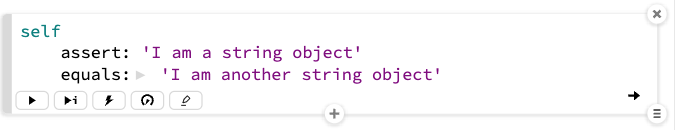
\includegraphics[width=\columnwidth]{stringComparisonSnippet}
  \caption{A failing string comparison assertion.}
  \label{fig:stringComparisonSnippet}
\end{figure}
In a normal setting, this assertion will fail, yielding a standard debugger view, such the one as we see in \autoref{fig:genericDebugger}.
\begin{figure}[h]
  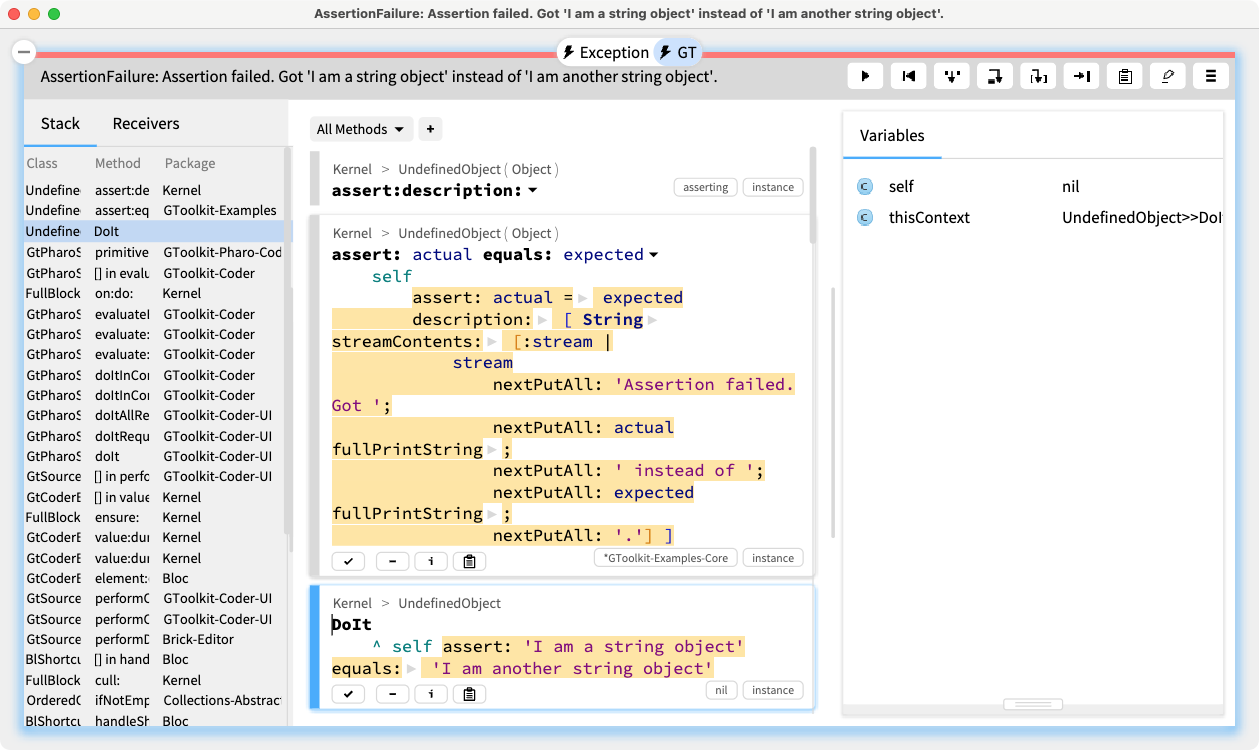
\includegraphics[width=\columnwidth]{genericDebugger}
  \caption{A generic debugger view.}
  \label{fig:genericDebugger}
\end{figure}
This is the standard debugger of the \GT IDE, which resembles other generic debuggers in that it shows an error message at the top, a compact view of the reified run-time stack at the left, source code of each stack frame in the middle, an inspector on the variables of the current stack frame at the right, and a dashboard of buttons at the top right for stepping through the running program.
It will typically take a developer some time to putter around in the debugger interface to understand the specific error (the strings do not match), and \emph{why} the strings do not match.

Suppose that instead of seeing the generic debugger, we are offered a view that highlights the actual differences, as in \autoref{fig:stringComparisonView}.
\begin{figure}[h]
  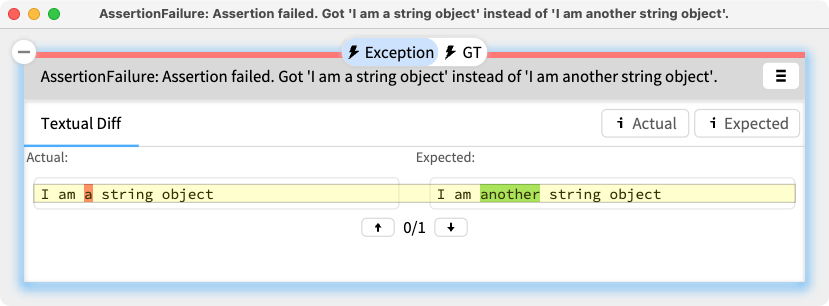
\includegraphics[width=\columnwidth]{stringComparisonView}
  \caption{A string diff debugger view.}
  \label{fig:stringComparisonView}
\end{figure}
Such a view not only homes directly in on the specific problem, but also highlights the individual differences in a dedicated ``diff'' view.
Furthermore, since the diff view already exists as a component used in other applications, the development effort is close to zero.
While in this introductory example, the difference is easy to spot, in other cases such as those presented in \autoref{sec:casestudy}, a diff view is essential to quickly identifying differences.

Moldable exceptions work as follows: when an exception is raised, the exception (an object) is caught and passed to the debugger.
Every exception not only provides the debugger with the context it needs to generate the debugging UI, but it can also offer alternative views and actions.
In the case of our implementation, this is achieved by the exception class providing specially annotated debugger extension methods.

This simple mechanism allows moldable exceptions to do three things:
\begin{enumerate}[(i)]
	\item provide domain-specific debugging views and actions,
	\item offer new debugger GUI interactions, and
	\item enable automated fixes (code and data transformations) for common programming errors.
\end{enumerate}

We will illustrate these three points with several examples.
In \autoref{sec:inspectorViews} we introduce the \emph{moldable inspector}, which allows objects to define custom views and actions when they are inspected.
In \autoref{sec:views} we show how custom debugger views can easily be defined in a similar way by adding simple annotated view and action methods to the class of a moldable exception.
In \autoref{sec:interactions} we show how a richer debugger user interface can be provided in much the same way by leveraging existing GUI frameworks.
We show an example of moldable exceptions enabling automated fixes in \autoref{sec:fixes}.
In \autoref{sec:casestudy} we describe a case study in which we used moldable exceptions to improve a development workflow.
We discuss the implementation details in \autoref{sec:implementation}.
We summarize our contributions and discuss some possible future work in \autoref{sec:directions}, and we discuss related work in \autoref{sec:related}.
We conclude in \autoref{sec:conclusion}.

% ============================================================
\section{The moldable inspector}\label{sec:inspectorViews}

Understanding moldable exceptions can be easier if we first introduce another example of a similar approach.
Moldable exceptions build on the idea of a \emph{moldable tool}~\cite{Chis17a}, an IDE tool that adapts its behavior to a specific run-time application context.
An example of such a tool is a \emph{moldable object inspector}~\cite{Chis15a}.
When a moldable object inspector is opened on an object it looks for any view or action methods defined in the class of that object, and uses those methods to create custom views.

Let us consider a typical example.
Suppose we have an implementation of a Ludo\footnote{A simple game in which players move tokens around a board based on the roll of a die.
\url{https://en.wikipedia.org/wiki/Ludo}} game.
Players alternate in throwing a die and moving a token until one player reaches their goal square.
In \autoref{fig:ludoRawView} we see a classical \emph{Raw} view supported by a typical object inspector.
\begin{figure}[h]
  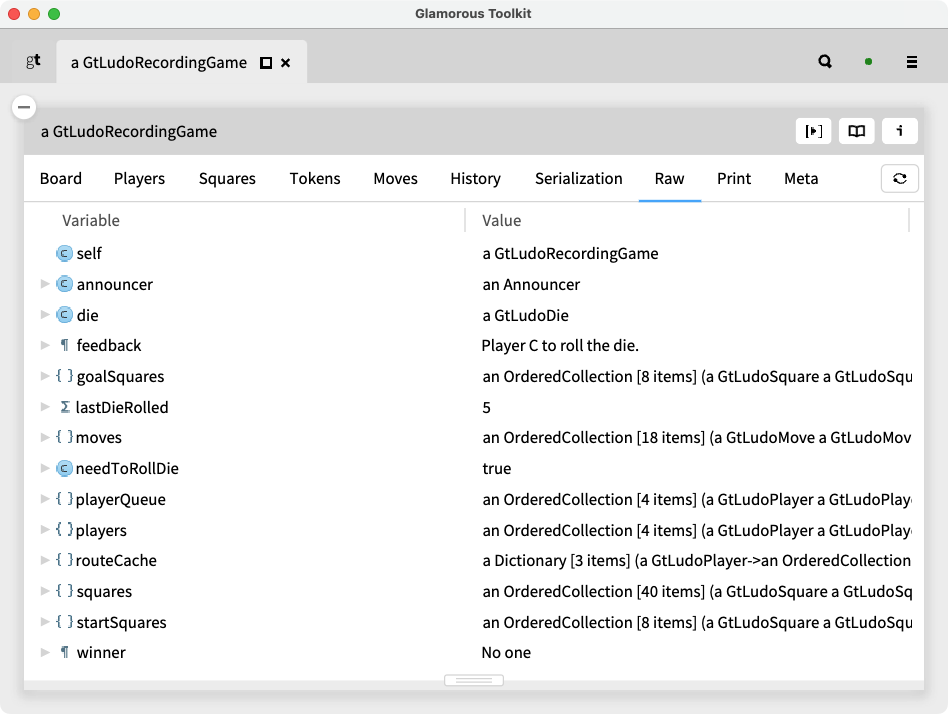
\includegraphics[width=\columnwidth]{ludoRawView}
  \caption{A classical ``raw'' view of a Ludo game.}
  \label{fig:ludoRawView}
\end{figure}
It just shows the state of the object as a list of instance variables and their values.
In \autoref{fig:ludoBoardView}, however, we see an alternative, graphical \emph{Board} view showing the current state of the game as a user would see it.
\begin{figure}[h]
  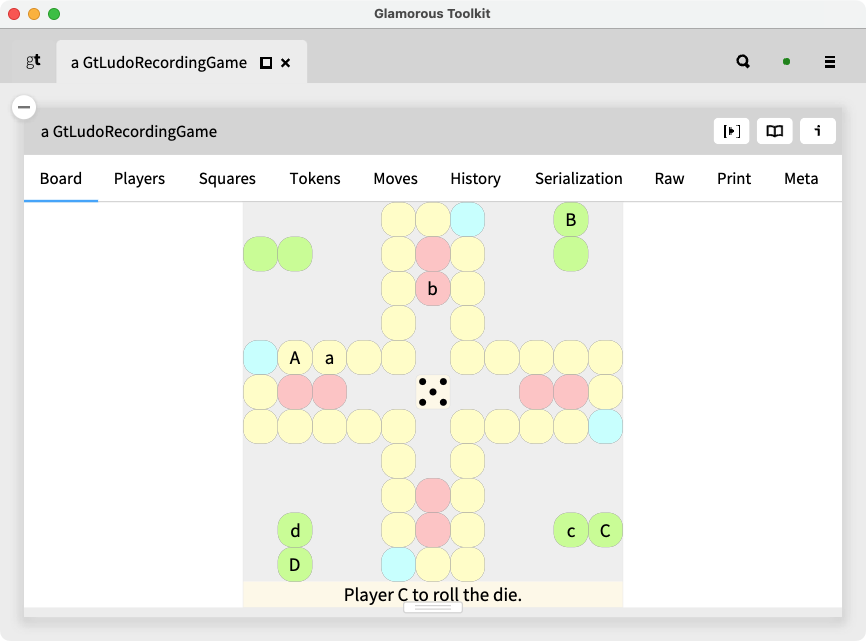
\includegraphics[width=\columnwidth]{ludoBoardView}
  \caption{An interactive GUI view of a Ludo game.}
  \label{fig:ludoBoardView}
\end{figure}

In general, a variety of views may be more useful than the classical ``raw'' view, and this is also true for the Ludo game.
In \autoref{fig:ludoMovesMoveViews} we see a \emph{Moves} view that lists all the moves of the game played thus far.
\begin{figure}[h]
  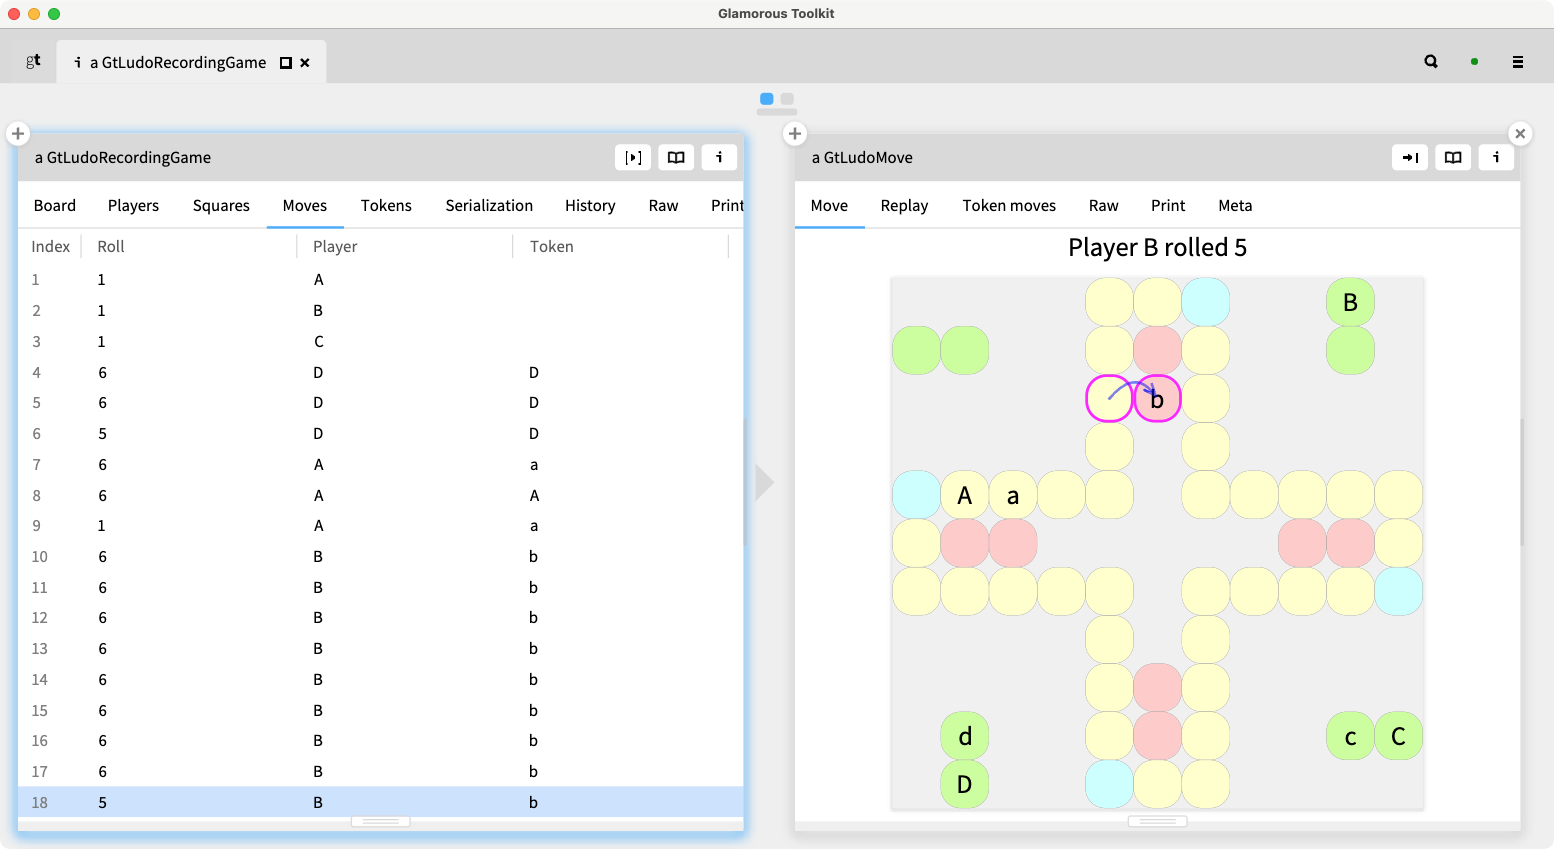
\includegraphics[width=\columnwidth]{ludoMovesMoveViews}
  \caption{A custom historical \emph{Moves} view of a Ludo game, and a custom graphical view of a selected move.}
  \label{fig:ludoMovesMoveViews}
\end{figure}
By clicking on a move (at the left) you can then inspect (at the right) the corresponding \st{GtLudoMove} object, with its custom views, in this case showing the details of what happened in this move.

In \autoref{fig:ludoMovesSource} we see the source code defining the \emph{Moves} view.
\begin{figure}[h]
  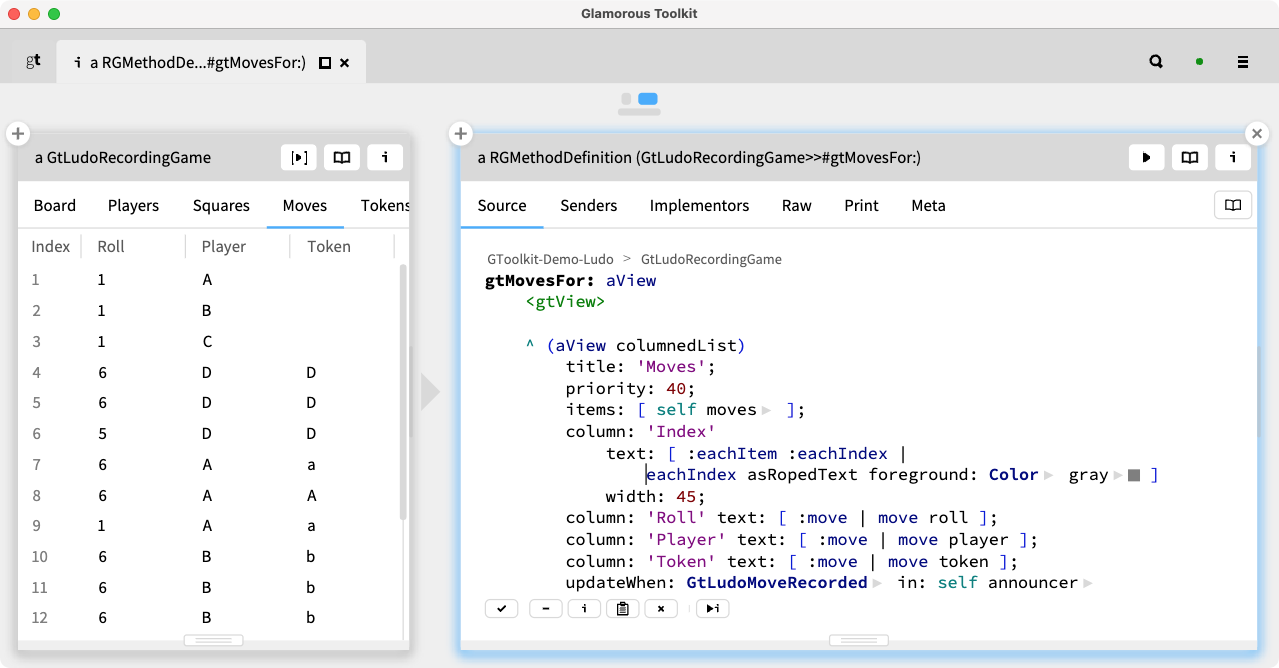
\includegraphics[width=\columnwidth]{ludoMovesSource}
  \caption{The \emph{Moves} view next to its source code.}
  \label{fig:ludoMovesSource}
\end{figure}
This method uses just a few lines of code to create a browsable ``columned list'' of past moves with several columns for the details of each move.

In addition to views, objects can also define \emph{actions} that encapsulate useful operations.
For example, the game object in \autoref{fig:ludoBoardView} defines a \lst{Autoplay one move} action with the icon \smallimg{ludoPlayActionIcon}) that can be used to simulate a player's turn.
%\ac{see later one how to get a less pixelated icon}

%\begin{code}
%gtAutoplayAction: anAction
%	<gtAction>
%	^ anAction button
%		tooltip: 'Autoplay one move';
%		priority: 20;
%		icon: BrGlamorousIcons go;
%		action: [ :aButton |
%			self autoPlay: 1.
%			aButton phlow spawnObject: self moves last ]
%\end{code}

View and action methods are recognized by the moldable inspector through dedicated annotations, in exactly the same way that a test runner tool in a classical IDE recognizes Java test case methods because they are tagged with a \st{@Test} annotation.
In this case the annotation is \st{<gtView>} for views and \st{<gtAction>} for actions, seen in the second line of the two defining methods.

% ============================================================
\section{Adding custom debugger views}\label{sec:views}

Moldable exceptions provide custom debugger views and actions in essentially the same way as the moldable inspector.
Moldable exceptions are instances of an \emph{Exception} class that has been extended with a dedicated method for each custom debugger view or action.
These methods are annotated with a \lst{<gtExceptionView>} pragma.

Let us consider that the Ludo game has been implemented with the help of \emph{Design by Contract}~\cite{Meye92b}.
Rolling a die when a player should move, or vice versa, constitutes a precondition violation, which raises a \st{LudoMoveAssertionFailure}.
Similarly, if an attempt is made to move the wrong player's token, this will trigger a precondition failure.
\begin{figure}[h]
  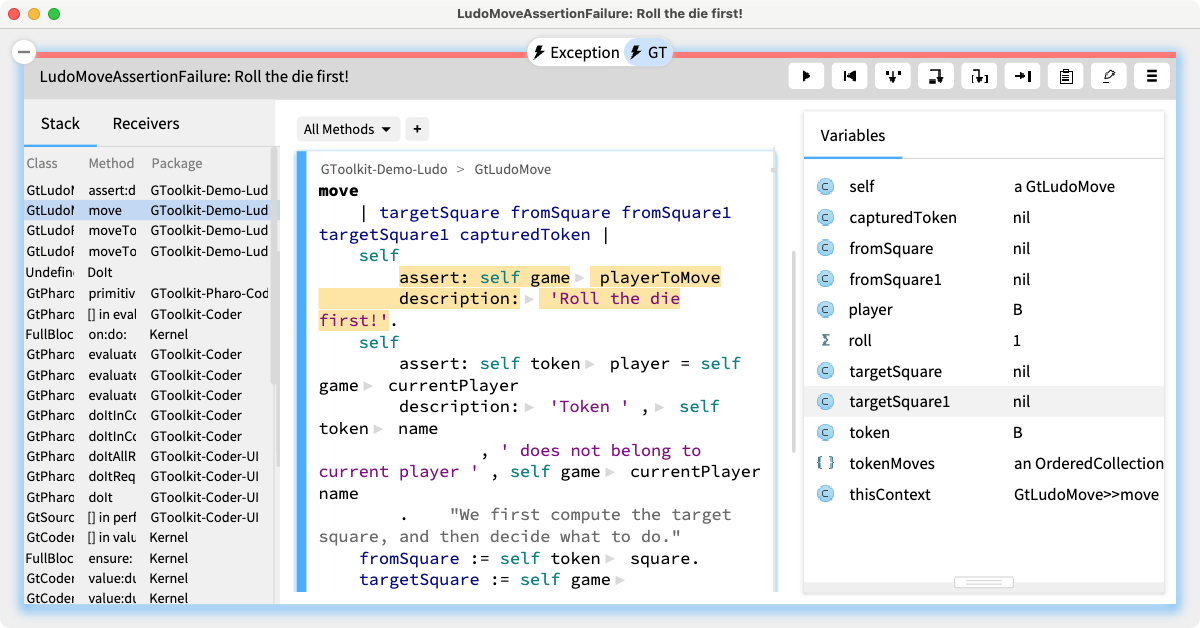
\includegraphics[width=\columnwidth]{ludoClassicDebugger}
  \caption{A classical debugger for a precondition failure.}
  \label{fig:ludoClassicDebugger}
\end{figure}
Normally, this would fire up the classical debugger, as seen in \autoref{fig:ludoClassicDebugger}.
Although the precondition violation is clearly reported, the debugger interface is not ideal for tracking down the actual reason for the violation.

What we would perhaps like to see instead is the current state of the game, in addition to a history of the past moves.
We could possibly find these by navigating through the existing debugger views, but why not show them directly?
After all, we know whenever this exception is raised, what it is that we would like to see.
Furthermore, if we already have such views defined elsewhere (we do!), it is not a question of defining new views, but of reusing them in the context of the debugger.
We just need to define two new view methods in the class \lmaf.

Here is the definition of the first view, which simply forwards (delegates) the view to another existing one.
\begin{code}
gtGameViewFor: aView
	<gtExceptionView>
	^ aView forward
		title: 'Game';
		priority: 10;
		object: [ move game ];
		view: #gtPositionsFor:
\end{code}

Let us step through the code:
\begin{inparaenum}[(i)]
	\item \st{gtGameViewFor:} is the name of the view method, which takes as its argument \lst{aView}, the view to be defined.
	\item The method is annotated with \lst{<gtExceptionView>}, which tells the moldable debugger to enable the view whenever \lmaf is raised.
	\item We return (\st{^}) the result of sending \st{forward} to \st{aView}.
	\item We give the view a title and
	\item a priority (order in which views ---  we set it to $10$ rather than $1$ to leave room for more important views later).
	\item We specify the object to forward to (the move's \st{game}).
	\item We name the already existing view method to forward to (\st{gtPositionsFor:}).
\end{inparaenum}

We similarly define a method for the history of past moves, and now the debugger, instead of showing us the classical debugger, will offer us the two views seen in \autoref{fig:ludoCustomViews}.
\begin{figure}[h]
  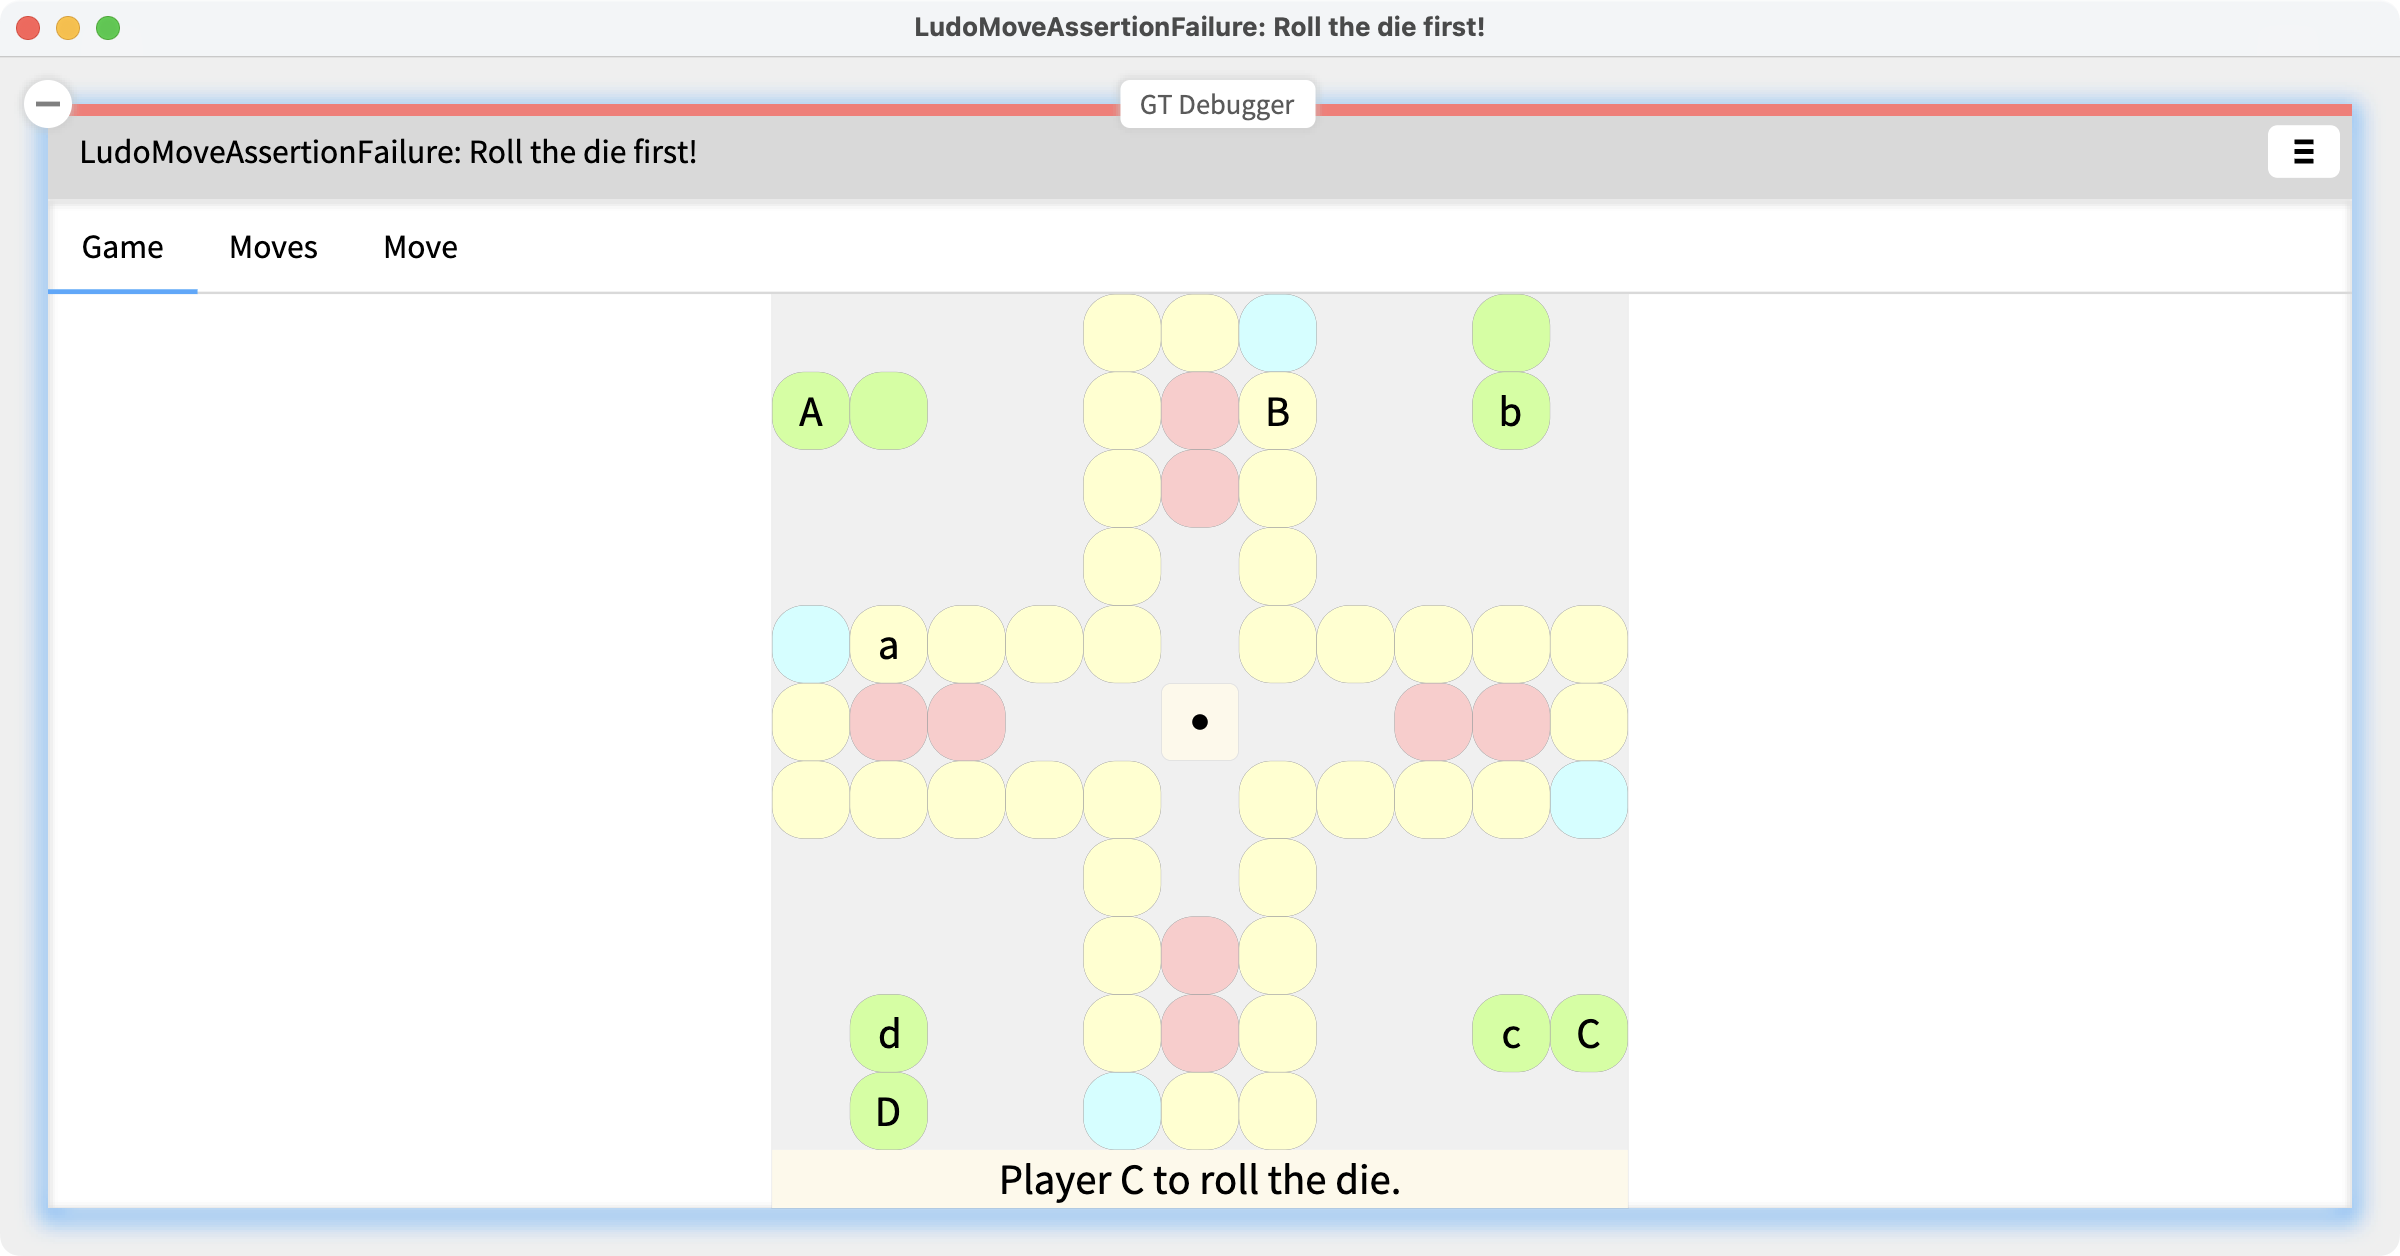
\includegraphics[width=\columnwidth]{ludoView1-Game}
  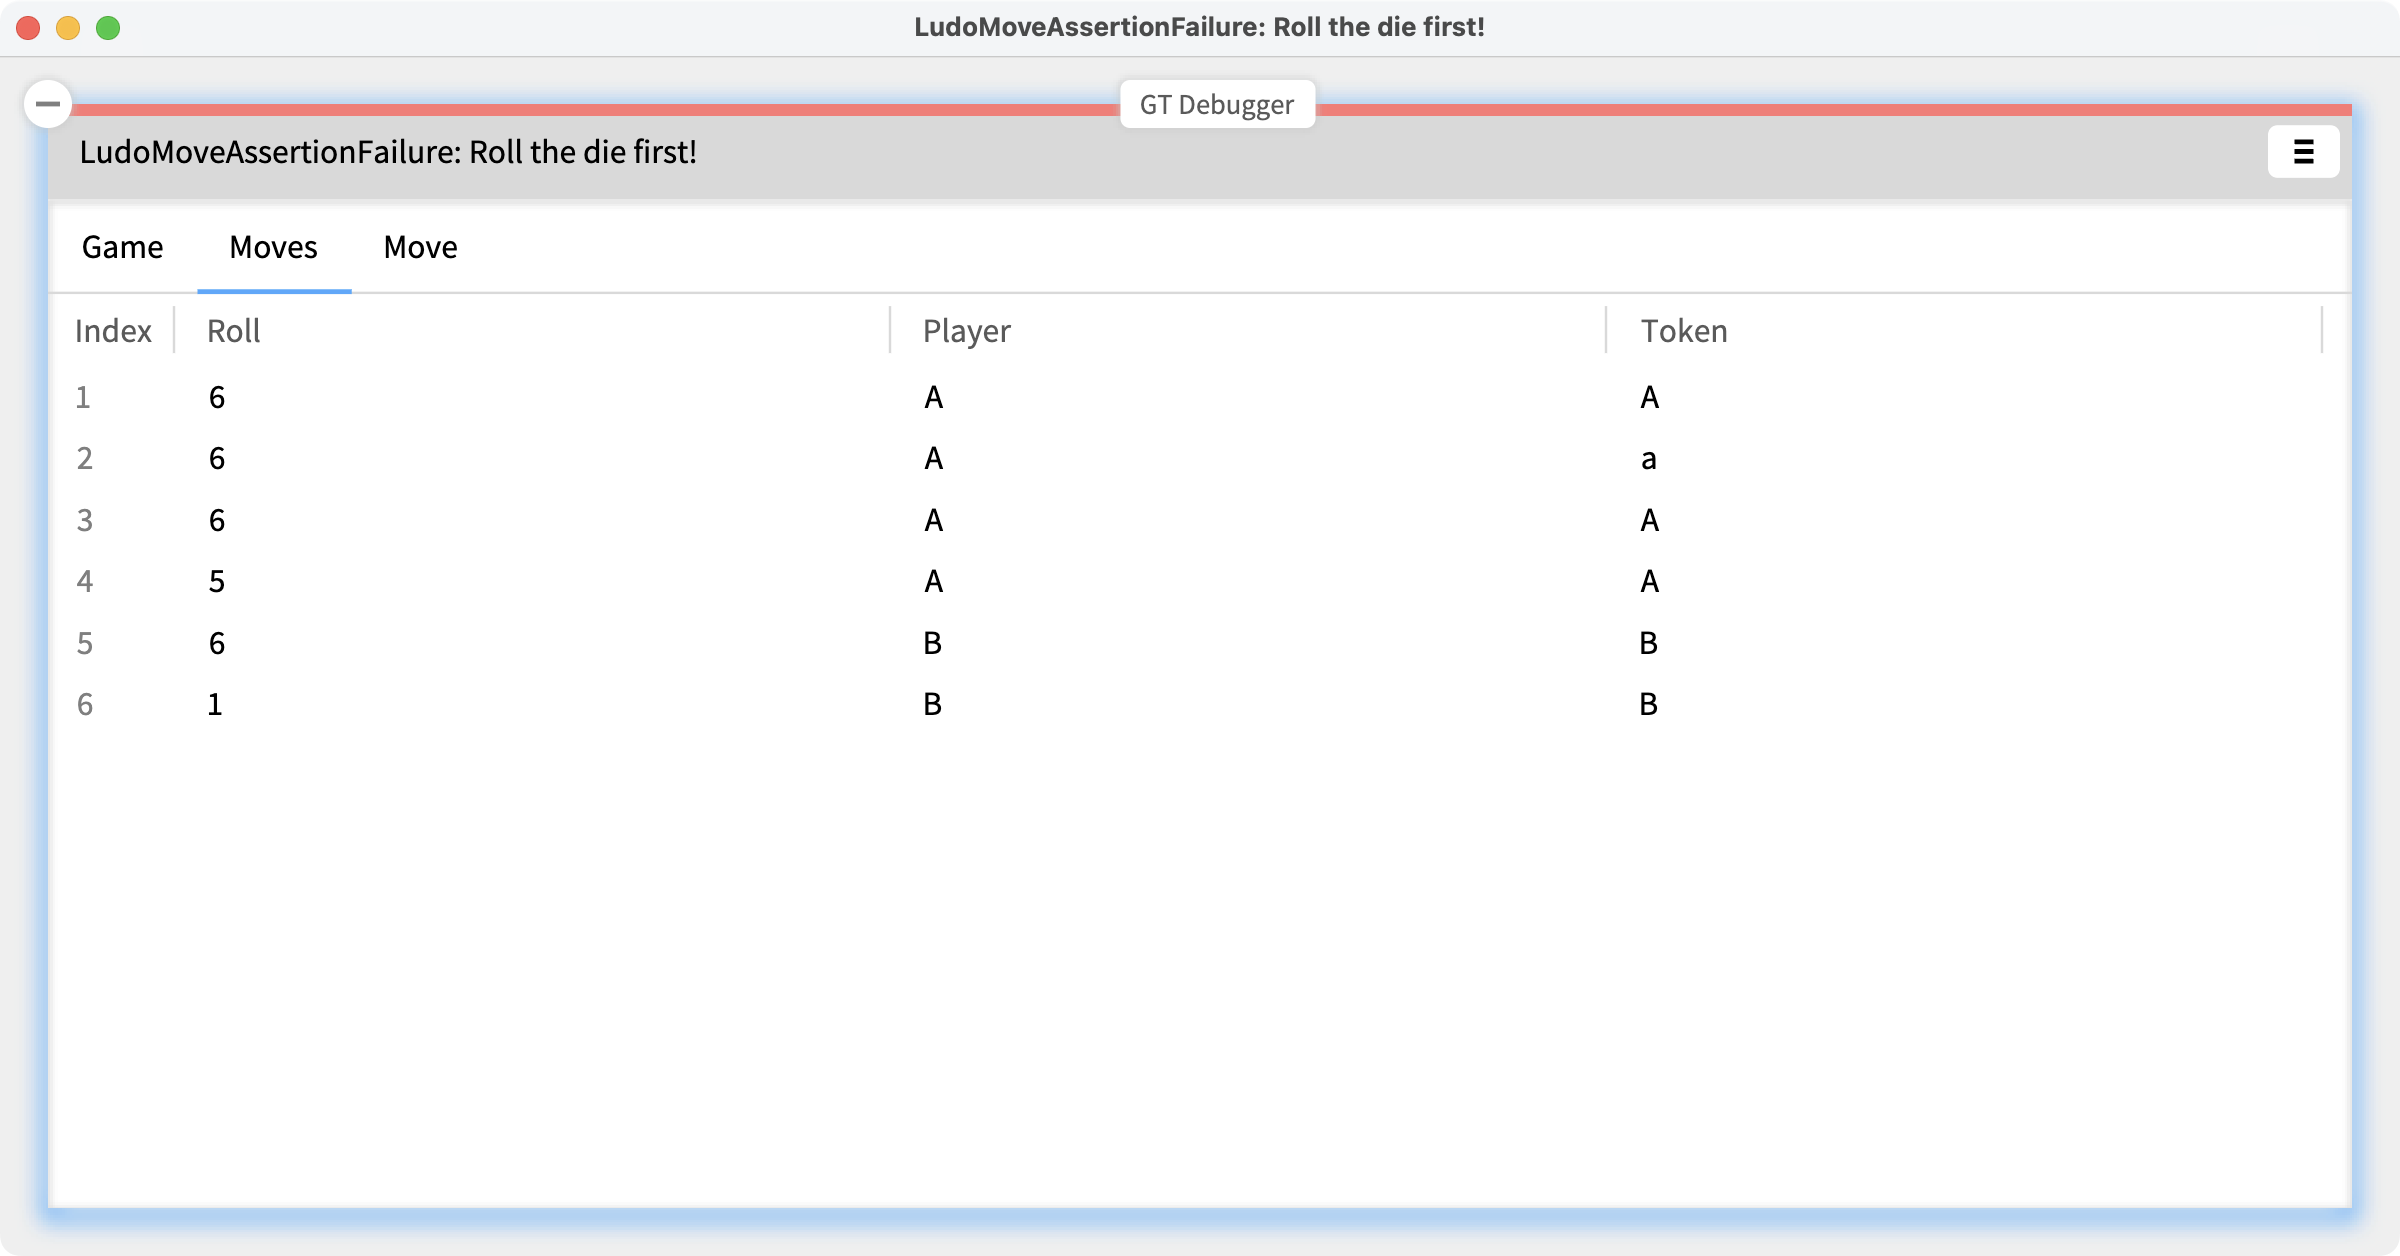
\includegraphics[width=\columnwidth]{ludoView2-Moves}
  \caption{Custom debugger views for the Ludo game.}
  \label{fig:ludoCustomViews}
\end{figure}
The Game view shows us the current game state graphically, and the Moves view shows us a browsable list of past moves.
Note that we can always switch to the standard debugger by selecting the \emph{GT} button at the top.

The \emph{Moves} debugger view is also defined by reusing the existing object inspector \emph{Moves} view:
\needlines{3}
\begin{code}
gtMovesViewFor: aView
	<gtExceptionView>
	^ aView forward
		title: 'Moves';
		priority: 20;
		object: [ move game ];
		view: #gtMovesFor:
\end{code}

The assertion diff debugger view we saw earlier in \autoref{fig:stringComparisonView} is similarly defined as a method of \st{AssertionFailure}.
\begin{code}
AssertionFailure>>gtComparableTypesTextualDiffFor: aView
	<gtExceptionView>
	| assertionContext |
	self gtHasStack ifFalse: [ ^ aView empty ].
	assertionContext := self gtLocateAssertEqualsContextWithComparableTypes.
	assertionContext ifNil: [ ^ aView empty ].
	^ aView forward
		title: 'Textual Diff';
		priority: 0;
		object: [ assertionContext ];
		view: #gtComparableTypesTextualDiffFor:
\end{code}
The key difference is that not every \st{AssertionFailure} is raised as the result of a comparison.
For this reason, in line $6$, the view will be suppressed (\st{^ aView empty}) in case the assertion did \emph{not} fail in the context of an \st{assert:equals:} check.

% ============================================================
\section{Building domain-specific debugger views}\label{sec:interactions}

The examples we have seen so far have reused existing inspector views, but sometimes there is a need to develop a new kind of debugger view.
This also need not necessarily imply a heavy implementation effort.

The \GT \emph{Scripter} is a tool used to ``script'' GUI interactions, mainly for testing purposes.
Let us consider the case of assertion errors being raised while testing a user interface interaction with the help of the Scripter.
The scenario is the following:
\begin{inparaenum}[(i)]
	\item We create a notebook page called ``Page One''.
	\item We add a text snippet with a link to the \st{Object} class.
	\item We assert the existence of the page.
	\item We click the link.
	\item We check that a new page is created (\ie the \emph{Coder} for the \st{Object} class).
\end{inparaenum}
In case something goes wrong, we would like the debugger to provide us with high-level views of the state of the Scripter.

We consequently introduce three dedicated debugger views.
The \emph{Scripter preview} (\autoref{fig:scripterPreview}) shows the result of the scripted interaction:
\begin{inparaenum}[(i)]
	\item the notebook page has been created, containing a link to the class \st{Object}, and
	\item the link to the class has been clicked, opening a source code browser on the class.
\end{inparaenum}
\begin{figure}[h]
  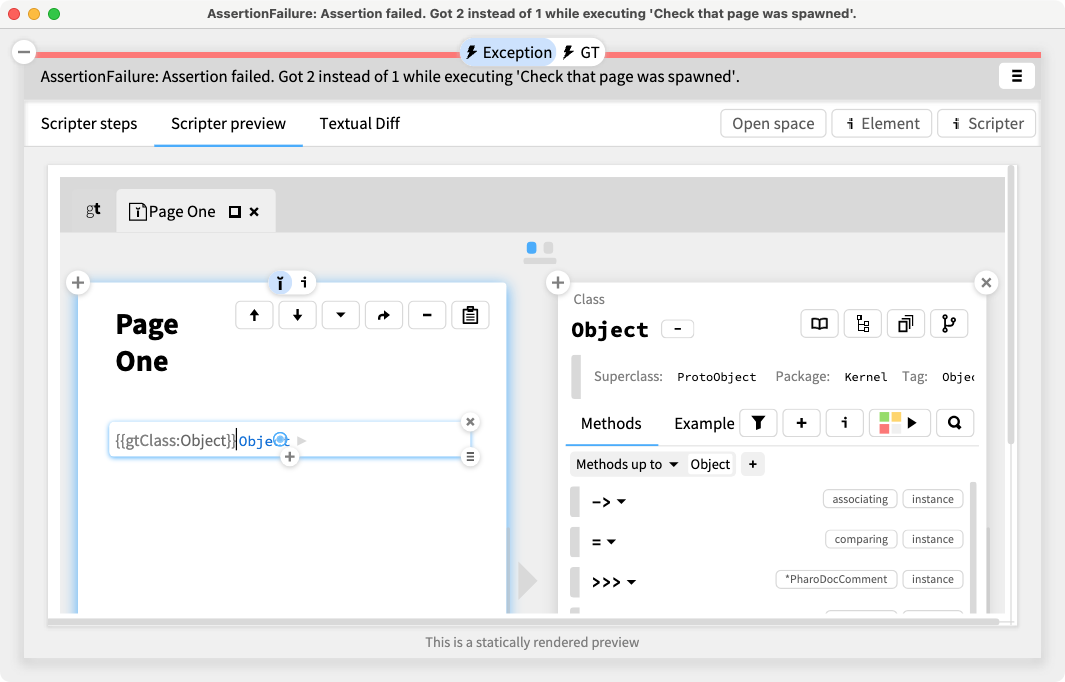
\includegraphics[width=\columnwidth]{scripterPreview}
  \caption{Scripter preview.}
  \label{fig:scripterPreview}
\end{figure}

The \emph{Scripter steps} view (\autoref{fig:scripterStepsViewClicked}) shows us a graphical tree view of the steps performed by the GUI Scripter, as well as the assertions that have been checked.
(In this case the tree has only two levels, but in general there may be many levels.)
\begin{figure}[h]
  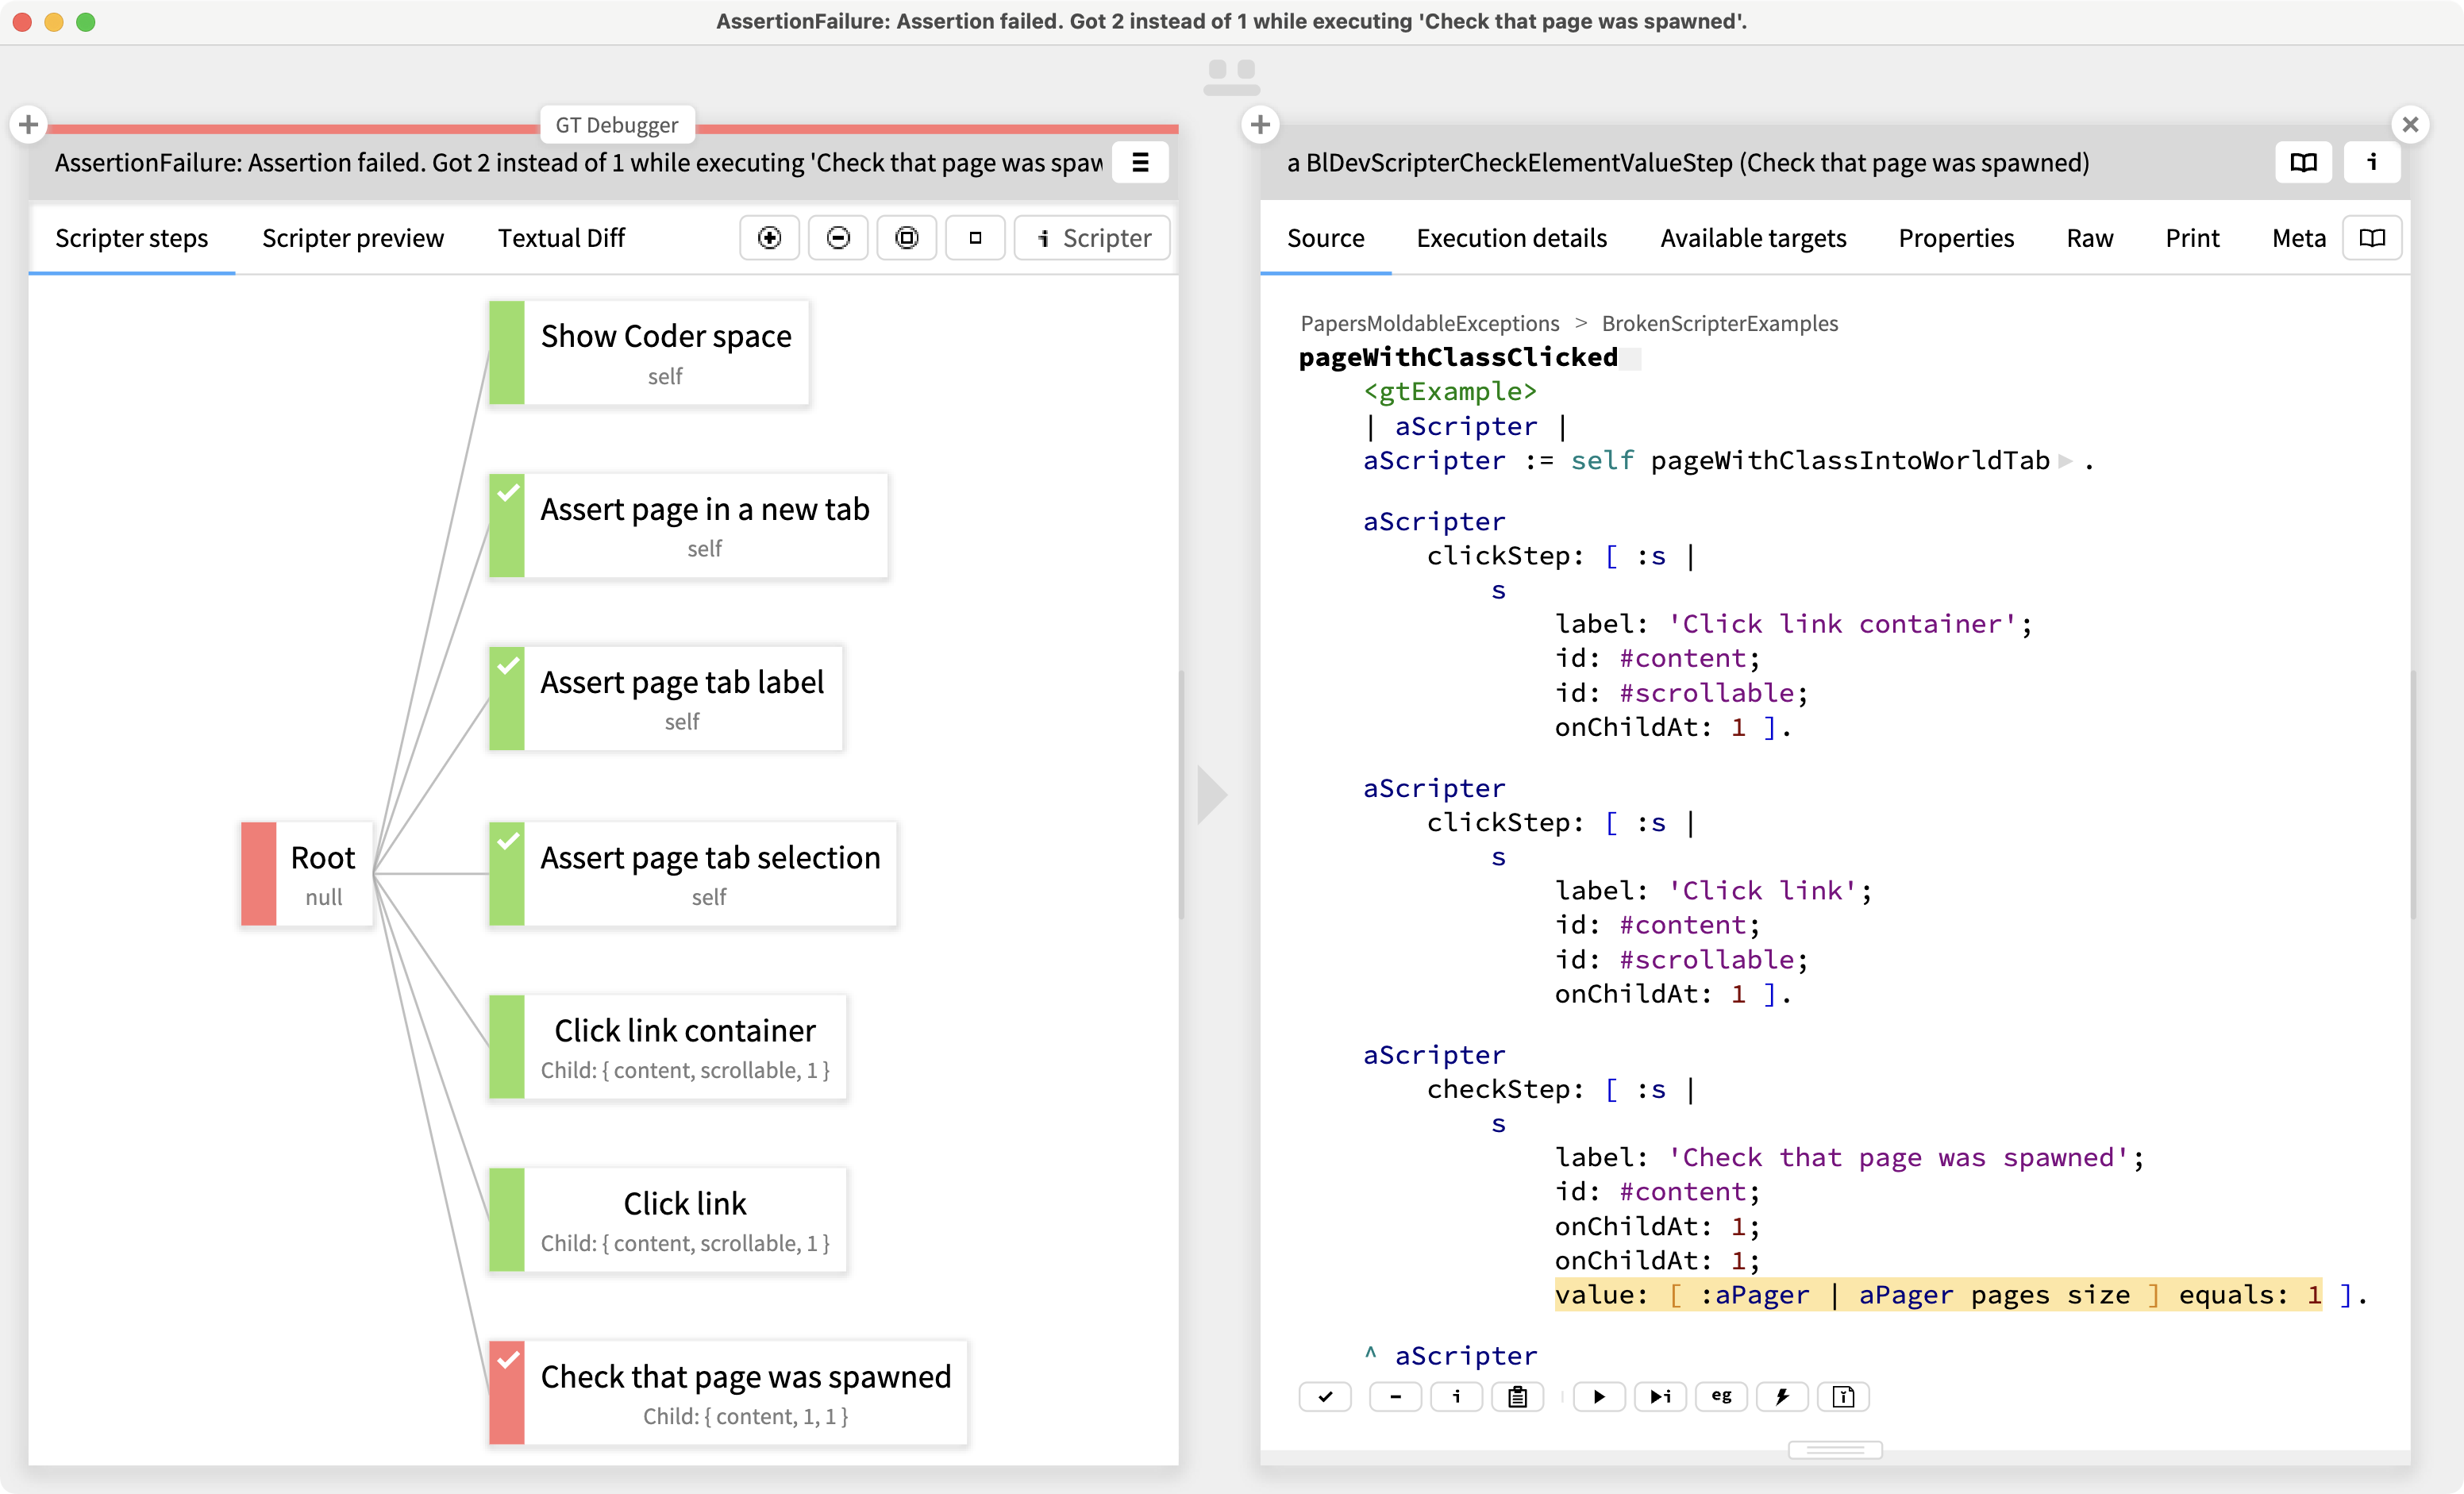
\includegraphics[width=\columnwidth]{scripterStepsViewClicked}
  \caption{Scripter steps view.}
  \label{fig:scripterStepsViewClicked}
\end{figure}
The green steps and assertions have succeeded, whereas the red ones have failed.
By clicking on any step or assertion node, we can see the corresponding code highlighted in the scripter method at the right.
Here we see that the step \emph{Check that page was spawned} has failed, and at the right we see the corresponding failure highlighted in the code.

Finally, the \emph{Textual Diff} view (\autoref{fig:scripterDiffInDebugger}) is the same one we have seen earlier, reused again.
\begin{figure}[h]
  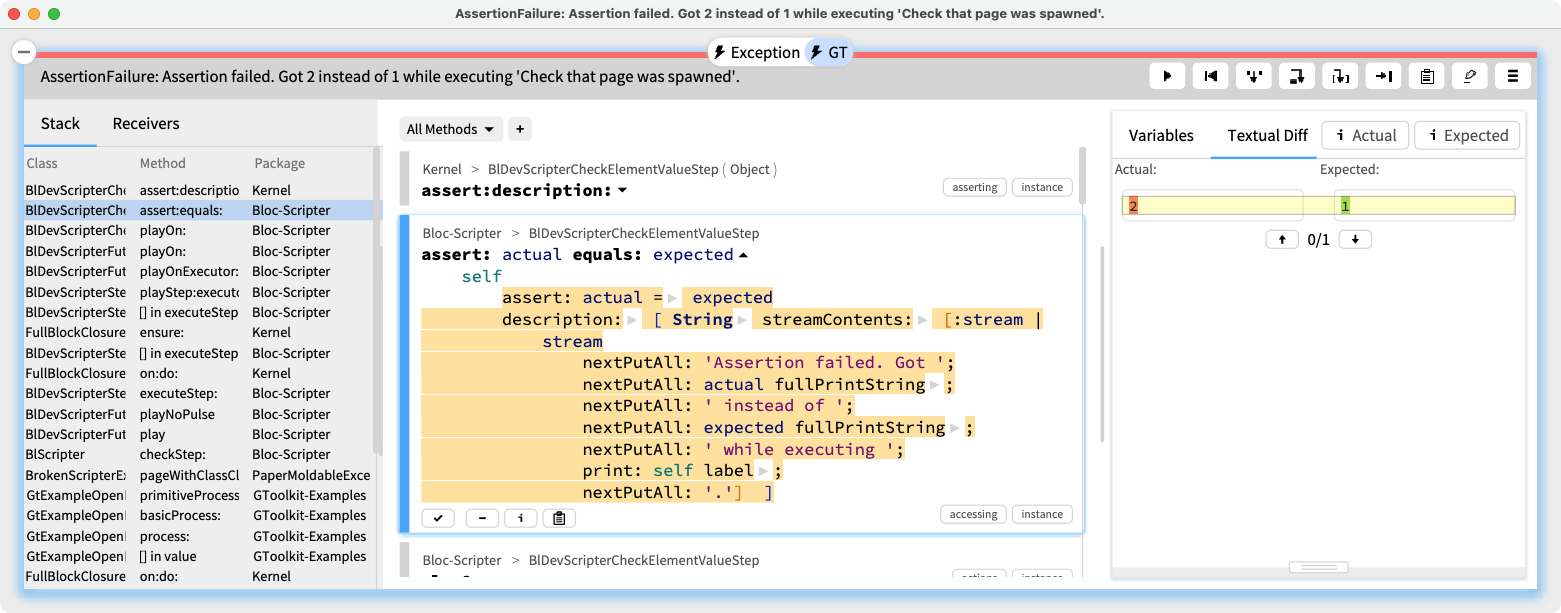
\includegraphics[width=\columnwidth]{scripterDiffInDebugger}
  \caption{Scripter textual diff view.}
  \label{fig:scripterDiffInDebugger}
\end{figure}
It just tells us that the check should verify that there are now two pages in the pager, not just one, as we can also see in the \emph{Scripter preview}.
It is the check specification that is at fault, not the GUI Interaction we are testing.

However this time we show the \lst{Textual Diff} view both in the new debugger interface created for this exception (\lst{Textual Diff} tab in \autoref{fig:scripterPreview}), as well as an additional view within the standard \GT debugger \GT debugger (\lst{Textual Diff} tab in \autoref{fig:scripterDiffInDebugger}).
Hence, a moldable exception can also provide views and actions shown in the standard \GT debugger.

\paragraph{Why do we need these views?}
The problem with the standard debugger is that, due to the way the GUI Scripter schedules the steps, the offending method (\ie the \lst{page\-With\-Class\-Clicked} method we see in \autoref{fig:scripterStepsViewClicked}) is \emph{not on the stack} at the point where the exception is raised.
Although it is possible to get at the information we seek, doing so is clumsy, and the classical stack view only confuses matters instead of helping us to debug the problem.
This can be the case with many application domains, especially those that depend on event scheduling.
The run-time stack does not do a good job of telling us how the events have been triggered, so another kind of view is needed.

\paragraph{How hard is it to implement a domain-specific debugger interface?}
Extending a standard debugger with such views can be challenging.
Typically such views would have to be added in a subclass of the standard debugger.
With moldable exceptions, views only have to be added to the exception class itself.
The \emph{Scripter steps view} is implemented using a version of \emph{Mondrian}~\cite{Pena13b,Meye06a}, a builder for graph-based visualizations.
In \autoref{fig:scripterStepsViewSource} we can see the entire source code of the view expanded in place, implemented in just four methods.\footnote{NB: The figure is intended just to emphasize the size of the source code, not to be an invitation to try to read it.}
\begin{figure}[h]
  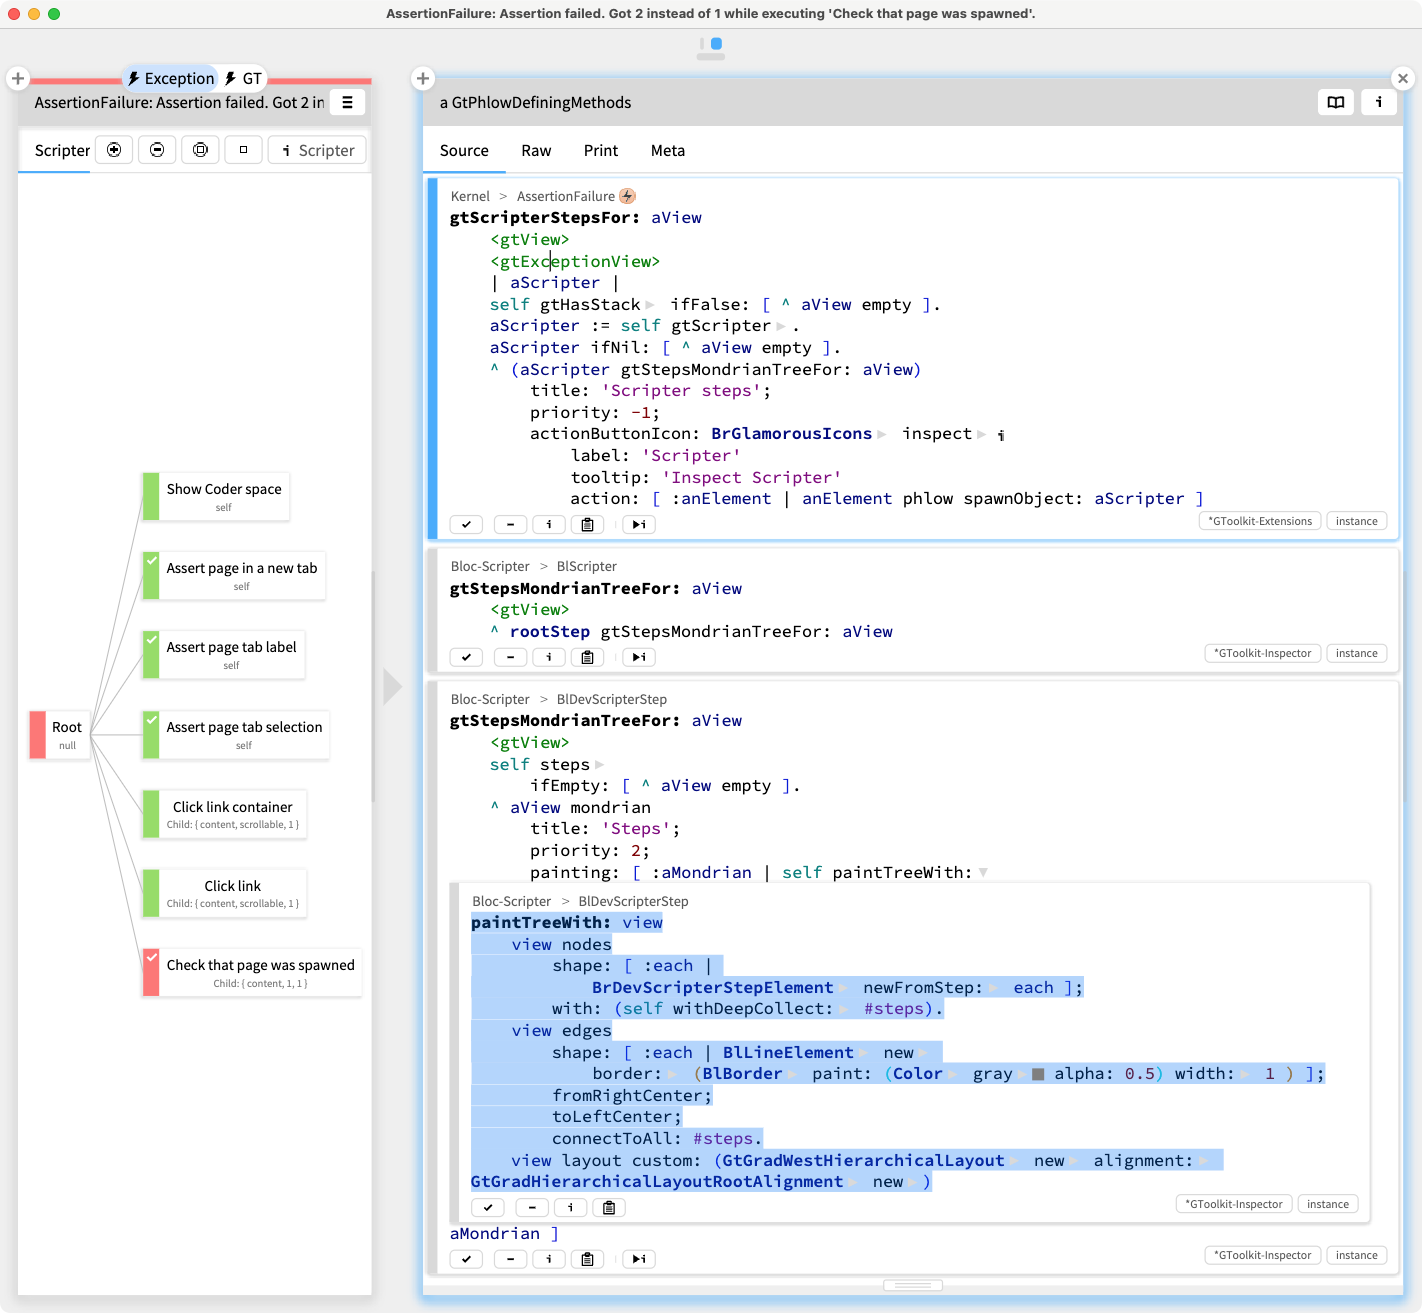
\includegraphics[width=\columnwidth]{scripterStepsViewSource}
  \caption{The Scripter steps source code.}
  \label{fig:scripterStepsViewSource}
\end{figure}
The debugging view at the top just adds a ``Inspect Scripter'' button to the next method, an object inspector view for a Scripter.
This in turn just delegates to the \emph{Steps} view of a \st{BlDevScripterStep} object.
Finally, this method embeds a Mondrian visualization implemented in 12 lines of code in the \st{paintTreeWith:} method.

Obviously this does not prove that all domain-specific debugger interfaces will be so tiny, but it does demonstrate that a useful custom debugger view can be implemented in an almost trivial amount of code.

% ============================================================
\section{Enabling automated fixes}\label{sec:fixes}

Many cases of common programming errors can be automatically repaired.
A good example is that of deprecated methods for which a well-defined alternative is available.
In Pharo Smalltalk this is achieved with the \lst{\#de\-pre\-cat\-ed:trans\-form\-With:} message defined in the \st{Object} class~\cite{Duca22a}.
It takes as arguments
\begin{inparaenum}[(i)]
	\item an explanatory string, and
	\item a source code transformation rule.
\end{inparaenum}
We see an example below, where the method \st{ClassDescription>>definition} has been deprecated, and should be replaced by \st{definitionString} in client code.
\begin{code}
ClassDescription>>definition
	"Answer a String that defines the receiver."
	self
		deprecated: #definition
		transformWith: '`@receiver definition' -> '`@receiver definitionString'.
	^ self definitionString
\end{code}
While the \st{deprecated:} message normally spawns a Debugger, in case a transformation rule is supplied, instead the client code is automatically rewritten, after which execution proceeds.
Here the transformation rule matches a send of \st{definition} for some receiver expression, and rewrites the message send to \st{definitionString}.

The fix is so straightforward, that it can be applied without any programmer intervention, or the need to spawn a debugger.
In \autoref{fig:deprecationDemo} we see the result of running client code of the old, deprecated method.
\begin{figure}[h]
  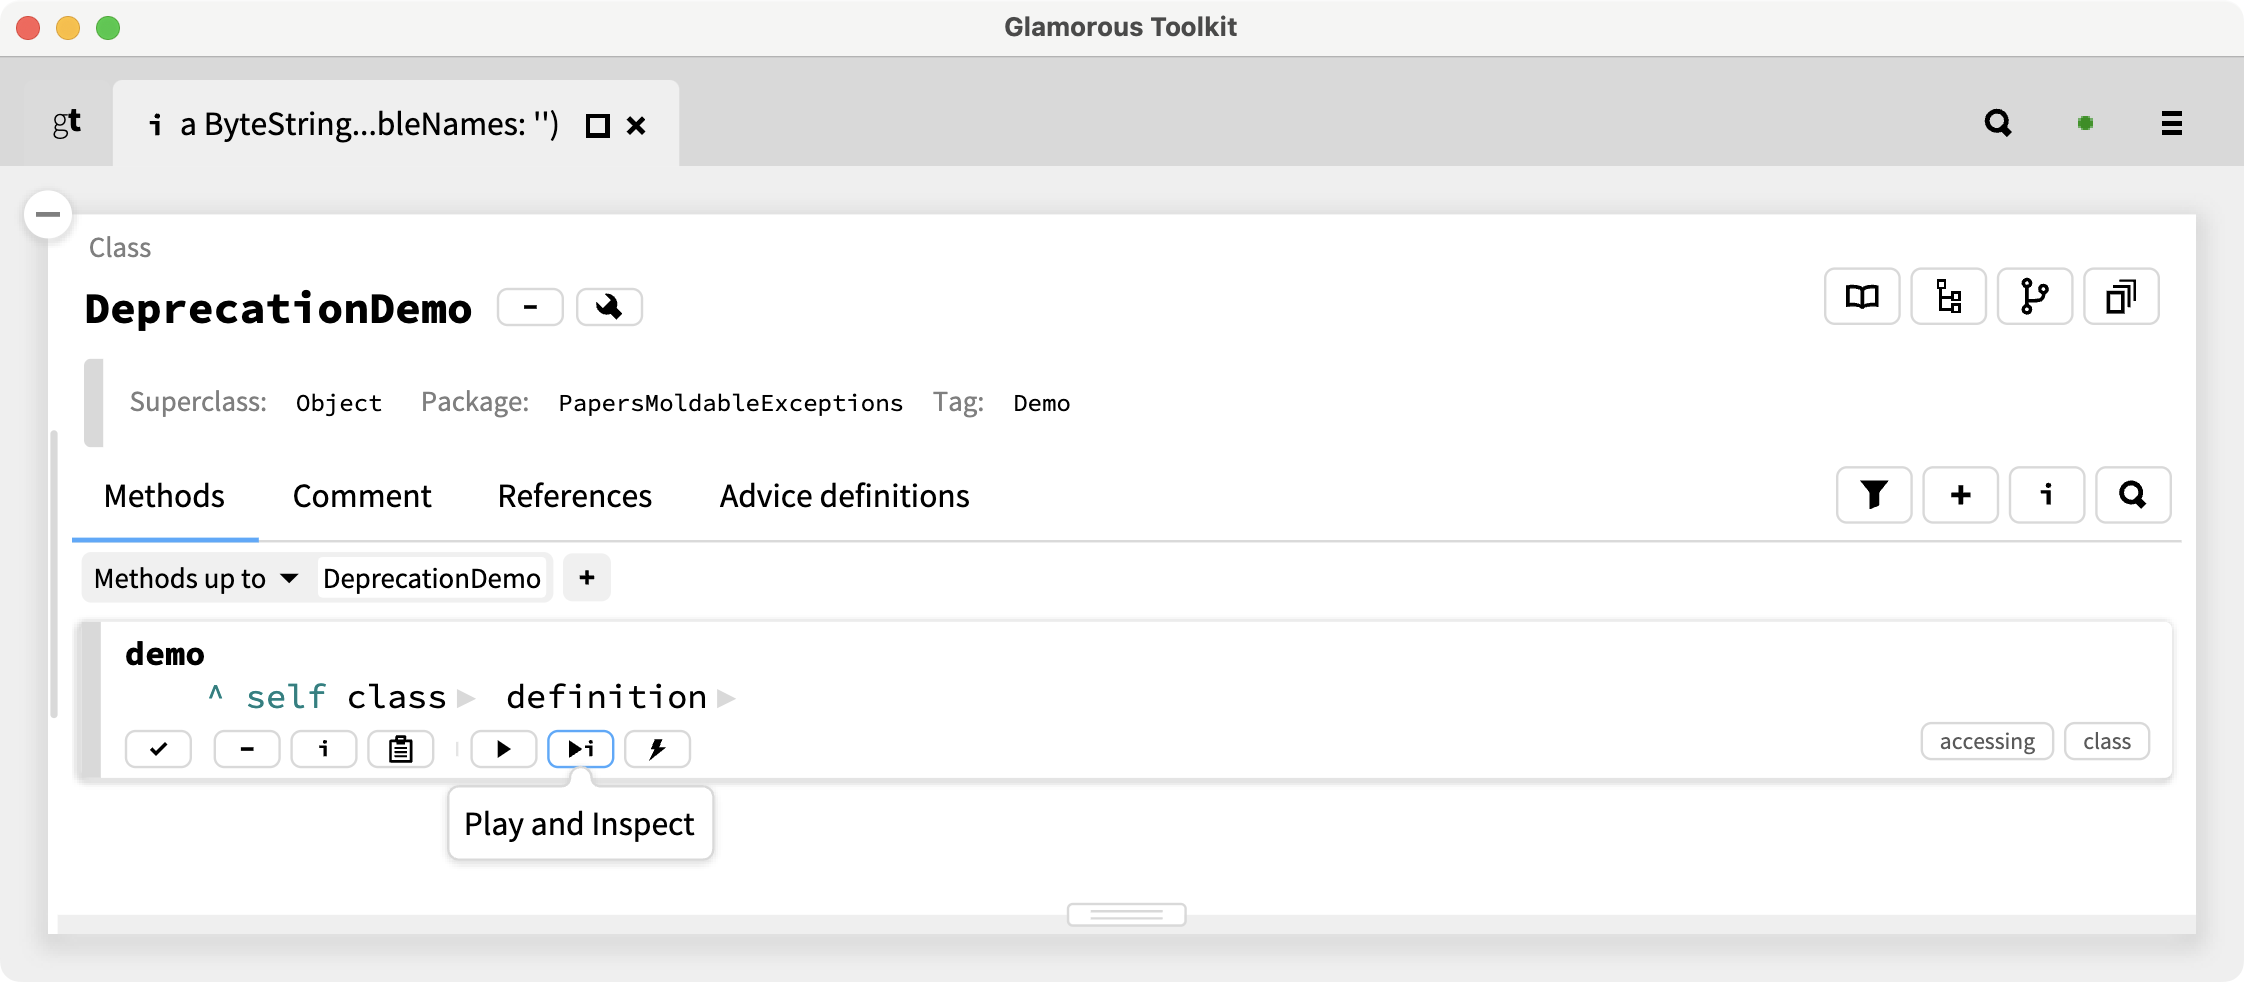
\includegraphics[width=\columnwidth]{deprecationDemoBefore}
  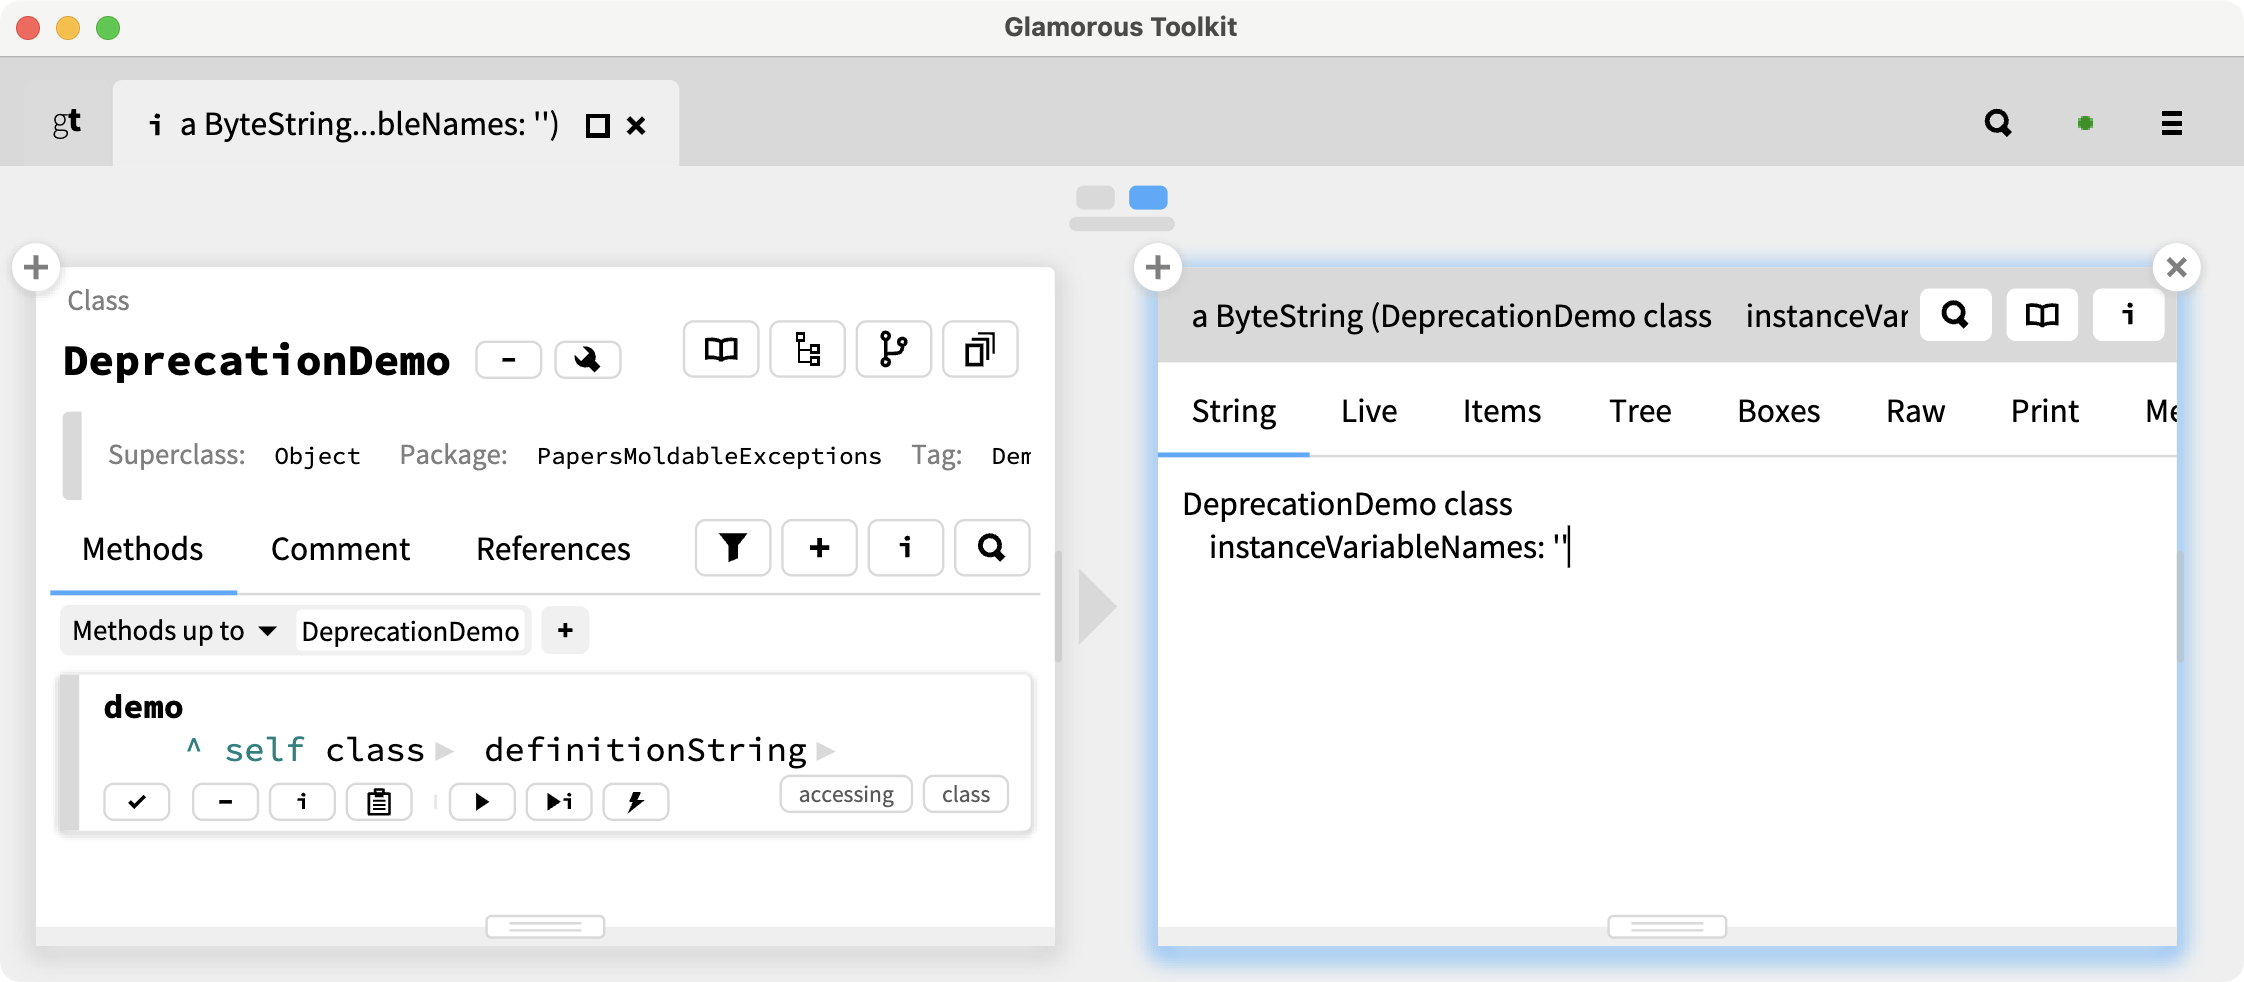
\includegraphics[width=\columnwidth]{deprecationDemoAfter}
  \caption{Automatically rewriting a client of deprecated code, before and after execution.}
  \label{fig:deprecationDemo}
\end{figure}
If we \emph{Play and Inspect} the method, we see that it is rewritten, and then directly evaluated.
(Compare the \st{demo} method bodies in the \emph{before} and \emph{after} screenshots.)

Unfortunately the automated fix for deprecated methods is bespoke behavior.
Pharo offers no general mechanism for automatically fixing other kinds of simple programming errors.
Moldable exceptions, however, offer a more general solution.

Consider the case of a common programming error being that of providing to an API an object of the wrong type, or of the right type but the wrong state.
While the first kind of mistake could arguably be caught a static type system, detecting objects being in a wrong state is rather a run-time issue, typically caught by a precondition.
Some common cases can be fixed by rewriting the client code.
In \autoref{fig:emptyViewError} we see the source code for a custom inspector view that incorrectly returns \st{aView} instead of \st{aView empty} in the preamble.
\begin{figure}[h]
  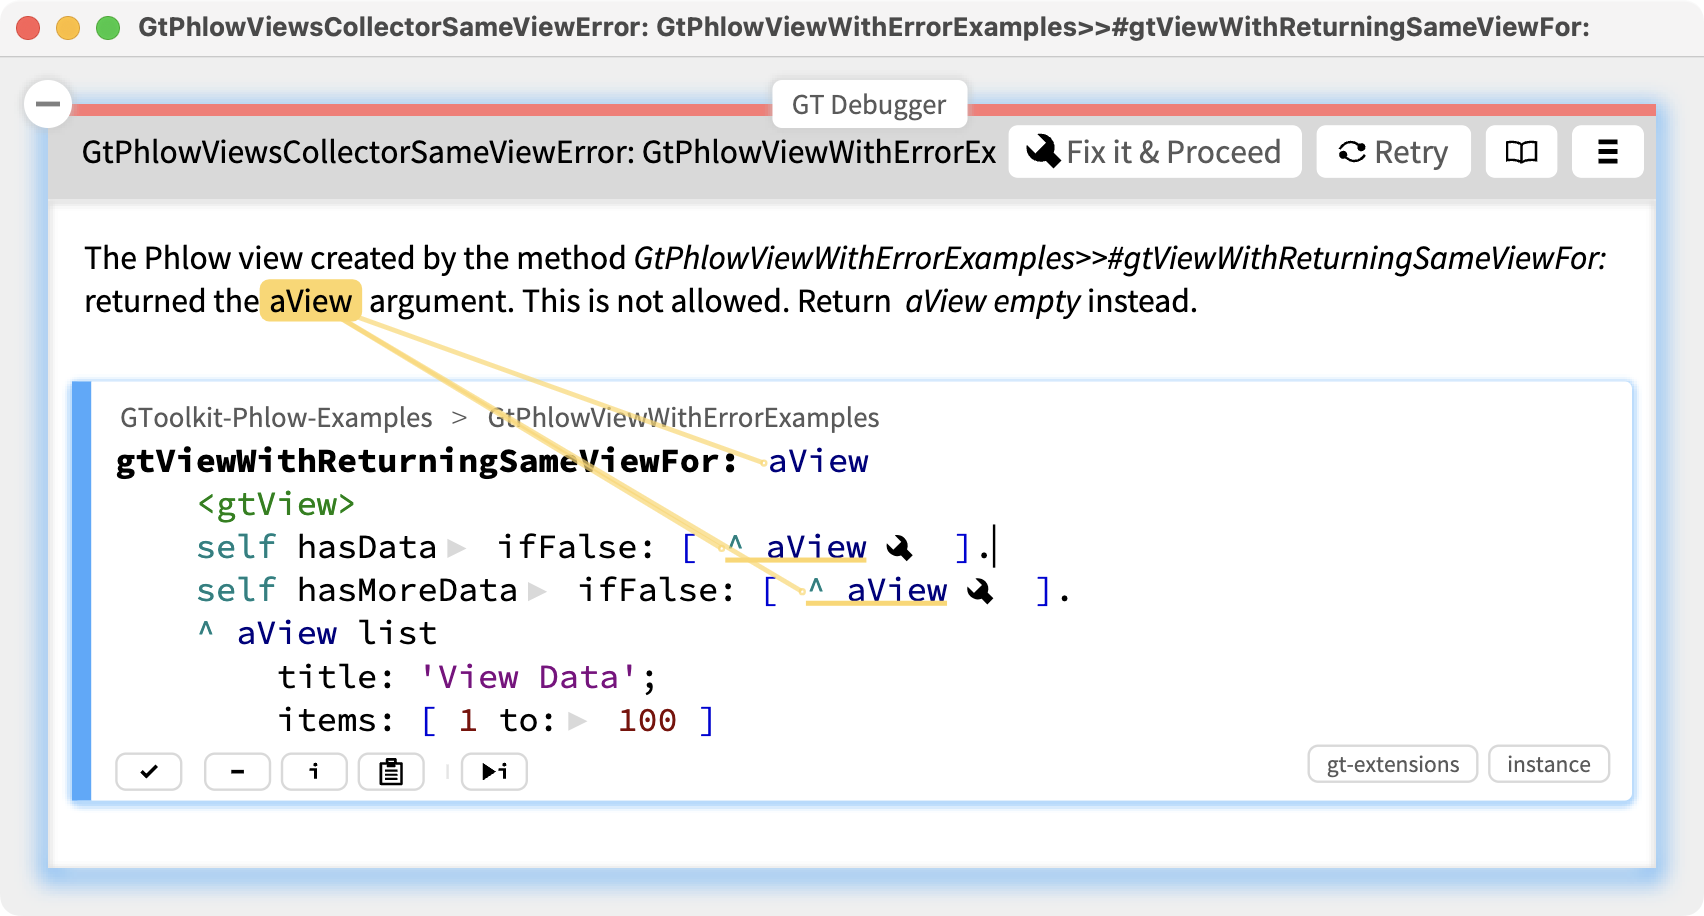
\includegraphics[width=\columnwidth]{emptyViewError}
  \caption{Catching an ``empty view'' error.}
  \label{fig:emptyViewError}
\end{figure}
This custom debugger view decorates the source code with an explanation pointing out the likely errors, and links (in yellow) to the offending source code.

Since such preambles are a common idiom in defining \GT inspector views, and the error is also not uncommon, it becomes easy to fix with the help of a transformation.
\autoref{fig:emptyViewErrorFix} shows the result of performing the \emph{Fix \& retry} action: a refactoring widget is generated that proposes a code transformation.
\begin{figure*}[h]
  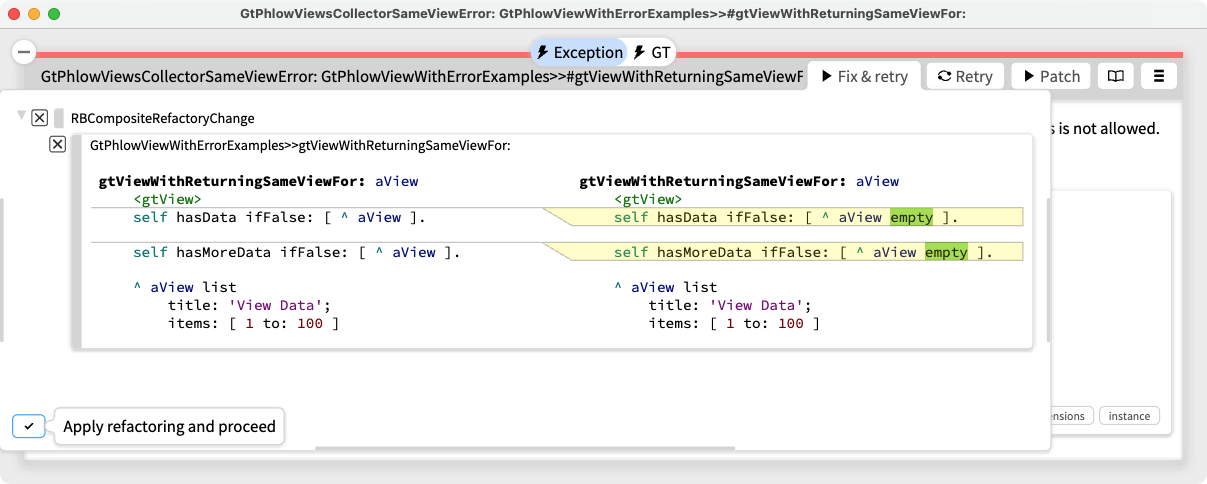
\includegraphics[width=\textwidth]{emptyViewErrorFix}
  \caption{Transforming an empty view error.}
  \label{fig:emptyViewErrorFix}
\end{figure*}
Clicking on the \emph{Apply refactoring and proceed} button will transform the source code, leave the debugger, and evaluate the rewritten code.

A custom debugger action, such as \emph{Fix \& retry} or \emph{Retry} is defined in the same way as a custom debugger view: it is a method with a particular annotation, in this case being \st{<gtPhlowSameViewReturnDebugAction>} rather than \mbox{\st{<gtExceptionView>}}, but  the mechanism is essentially the same.
We see the code of this action in the listing below.
Since this is a debugging action we need to be able to control the run-time execution.
To make this possible, methods creating debugging views and actions can take as a second parameter a context object that gives them access to the current run-time execution.

\begin{code}
gtDebugActionFixItFor: anAction inContext: aContext
	<gtPhlowSameViewReturnDebugAction>
	(self shouldApplyInContext: aContext )
		ifFalse: [ ^ anAction noAction ].
	^ anAction dropdown
		label: 'Fix & retry';
		icon: BrGlamorousVectorIcons play ;
		priority: 50;
		id: #'gtDebugAction-fixit';
		preferredExtent: 650@350;
		content: [ self refactoringElementWithAction: [
			aContext debuggingSession restartTopContext.
			aContext debugger resumeAndCloseDebugger ]]
\end{code}

The default behavior of such fixits is to open a debugger with the possibility of applying a proposed code transformation.
If, on the other hand, such code transformations should be applied automatically, this can be configured.
In our proof-of-concept implementation of moldable exceptions, this is done by evaluation the following code, which sets a flag in a globally accessible Singleton.
\begin{code}
GtMoldableExceptionTransformationsSettings defaultInstance allowAutomaticTransformations.
\end{code}
The \st{signal} method of exception classes can then optionally consult this flag to decide whether to spawn a debugger or apply the fix (\autoref{sec:implementation} gives more details).

As before, the custom debugger views and actions are mostly built from existing components, so the implementation effort is low.

% ============================================================
\section{A case study of Moldable Exceptions}\label{sec:casestudy}

As a case study, we applied moldable exceptions within a company that develops applications for managing insurance policies, to improve the development process by integrating custom comparison views into the debugger.

One part of the application consists in generating various documents related to insurance contracts.
The creation of documents is verified using tests that check that a recreated document matches an expected version that has been previously saved.
Whenever a comparison fails, a developer needs to assess the differences between the two documents, and then, in case those differences are justified, update the saved version with the recreated one, or in case they are not expected, track down and fix the root cause of the difference.

In the established workflow, a developer uses a dedicated tool to compare the recreated and the expected versions, and in case the difference is acceptable, update the expected document with the new one.
In case the difference indicates a bug, the developer has to run the test again using the debugger to explore the live execution.
With this workflow, developers have to choose the tool \emph{before} they run the test, which means that they typically need to run a test twice.
This can be a problem as some tests take minutes to run.

With moldable exceptions we integrated custom debugger views that show the differences between the recreated and the expected versions, and provide custom actions to update the expected document with the new one and resume executing the test, directly in the debugger.
To achieve this we rely on the fact that tests raise \lst{ComparisonFailure} exceptions when two documents do not match.

\begin{figure*}[h]
  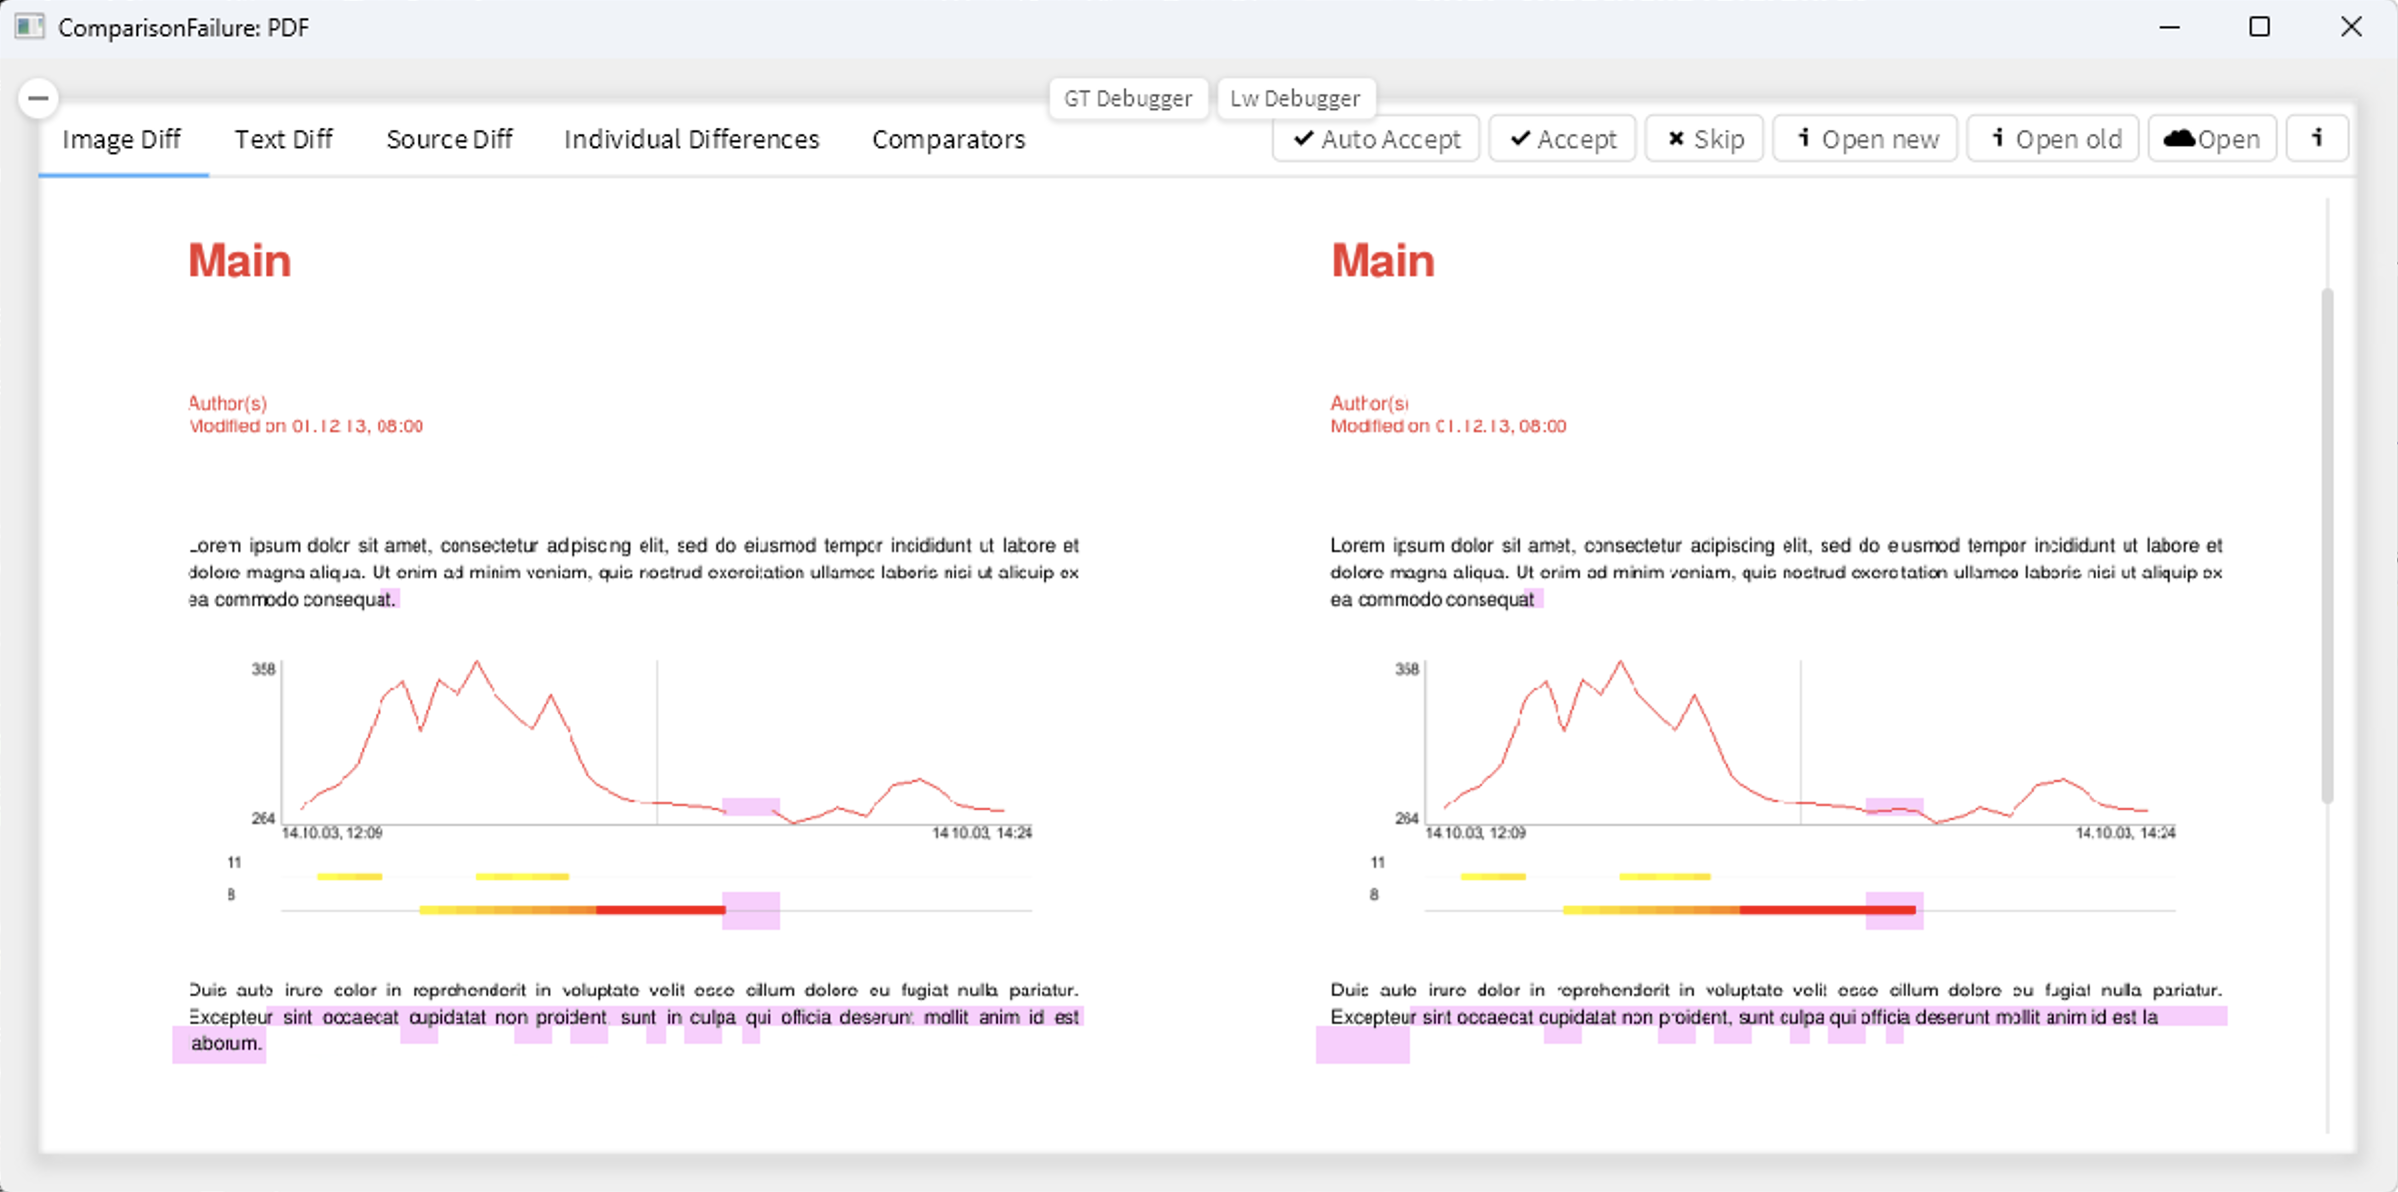
\includegraphics[width=\textwidth]{comparisonFailureVisualDiff}
  \caption{A view showing visual differences between two PDF documents (differences are highlighted in magenta).}
  \label{fig:comparisonFailureVisualDiff}
\end{figure*}

\begin{figure}[h]
  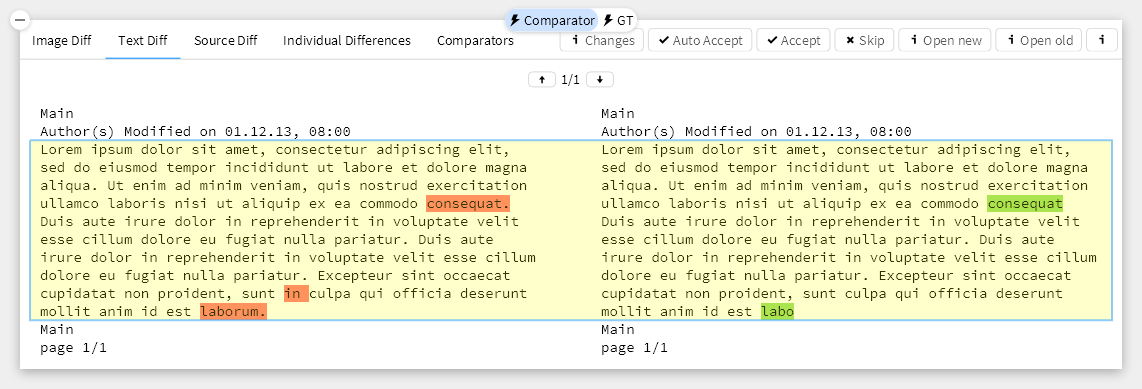
\includegraphics[width=\columnwidth]{comparisonFailureTextualDiff}
  \caption{A view showing textual differences between the text content of two PDF documents.}
  \label{fig:comparisonFailureTextualDiff}
\end{figure}

\begin{figure}[h]
  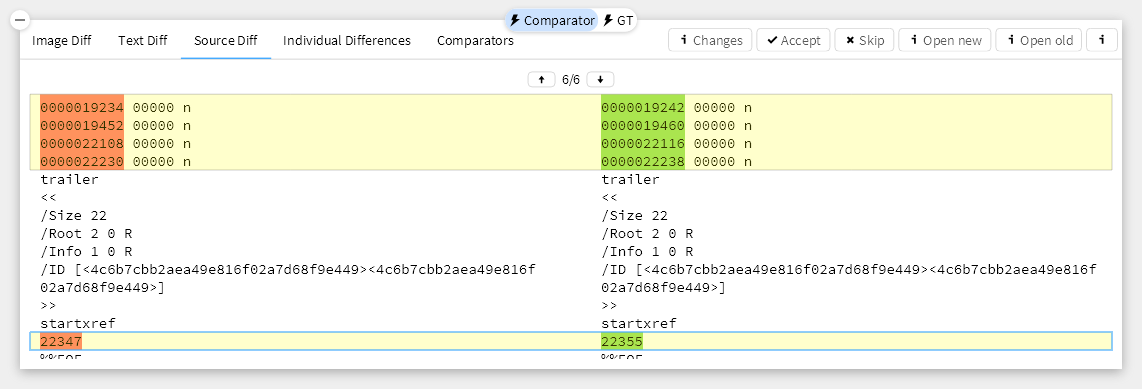
\includegraphics[width=\columnwidth]{comparisonFailureSourceDiff}
  \caption{A view showing textual differences between document at the level of the PDF format.}
  \label{fig:comparisonFailureSourceDiff}
\end{figure}


\autoref{fig:comparisonFailureVisualDiff} shows the debugger opened as a result of a failed comparison of two PDF documents.
In this case the exception provides multiple diff views:
one at the image level that visually highlights the parts that differ between the two documents (\autoref{fig:comparisonFailureVisualDiff}),
a second one at the level of the text contained by the PDF documents (\autoref{fig:comparisonFailureTextualDiff}),
and another at the level of the raw document format (\autoref{fig:comparisonFailureSourceDiff}).
Apart from the diff views, the exception also provides an \emph{Accept} action that replaces the saved expected document with the new one, and continues the execution of the test.

The \emph{Image Diff} view and the \emph{Accept} action both reuse existing logic, and in a few lines of code integrate it into the debugger.
This integration unifies the flow of comparing two documents and exploring why the failure happens using a debugger.
Developers can now simply run tests, and when a comparison fails choose how to proceed.

%Below we see respectively the source code of the \emph{Image Diff} view and the \emph{Accept} action.
%In both cases they reuse existing logic, and in a few lines of code integrate it in the debugger.
%This integration unifies the flow of comparing two documents and exploring why the failure happens using a debugger.
%Developers can now simply run tests, and when a comparison fails choose how to proceed.
%
%\begin{code}
%TextOrVisualComparisonType>>gtImageDiffFor: aView
%	<gtView>
%	<lwComparisonView>
%	self initialComparison = #visualComparison
%		ifFalse: [ ^ aView empty  ].
%	^(aView forward)
%		title: 'Image Diff';
%		priority: 8;
%		object: [ self createGtComparator ];
%		view: #gtViewImageDiffFor:
%\end{code}
%
%\begin{code}
%TextOrVisualComparisonType>>gtAcceptFor: anAction inContext: aContext
%	<lwComparisonAction>
%	aContext debuggingSession
%		isInterruptedContextPostMortem
%			ifTrue: [ ^ anAction noAction ].
%	^ anAction button
%		label: 'Accept';
%		icon: BrGlamorousVectorIcons accept ;
%		priority: 5;
%		id: #'lwComparisonAction-accept';
%		forViewDefinedIn: #gtImageDiffFor:;
%		action: [
%			aContext debugger
%				acceptCurrentTest;
%				resumeAndCloseDebugger ]
%\end{code}

% ============================================================
\section{Implementation details}\label{sec:implementation}

%We implemented the moldable exceptions idea in Glamorous Toolkit.
%This section discusses relevant aspects regarding its implementation.

The key to implementing moldable exceptions is the mechanism used to inform a moldable debugger of the relevant views and actions it provides.
% At the core of implementing moldable exceptions is allowing the exception to indicate how to locate relevant actions and views.
In our implementation every exception can provide one or more \emph{debugger specifications}.
Exceptions define these specifications through methods annotated with \lst{<gtDebuggerSpecification>}.
Below we see the method in the \lst{Exception} class, at the top of the exception class hierarchy, that defines a custom debugger for every exception.

\begin{code}
Exception>>gtExceptionDebuggerSpecification
	<gtDebuggerSpecification>
	^ GtMoldableExceptionSpecificDebuggerSpecification
		forException: self
\end{code}

A debugger specification contains all the information needed by a debugger to locate actions and views.
\autoref{fig:debuggerSpecificationsProperties} shows the default properties defined by such a specification.

\begin{figure}[h]
  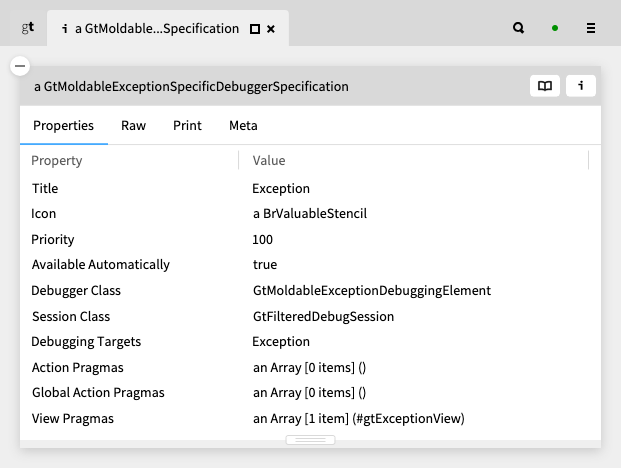
\includegraphics[width=\columnwidth]{debuggerSpecificationsProperties}
  \caption{Default properties for a debugging specification.}
  \label{fig:debuggerSpecificationsProperties}
\end{figure}

By default, as mentioned in \autoref{sec:views}, the moldable \GT debugger looks for methods annotated with a \lst{<gtExceptionView>} pragma.
An exception can change the pragma if needed, or provide a list of other pragmas.
The default specification also provides several other properties, including:
\begin{itemize}
\item Debugging Targets: objects reachable from the exception where to look for actions and views.
\item Debugging Actions: pragmas for debugging actions.
\item Title, Icon: for displaying a debugger selector.
\item Priority: a number used to determine the order in whichalternative debuggers are offered.
% debuggers are sorted by priority when shown; the lowest numbered one is selected first.
\item Activation Predicate: a condition to decide whether to show the debugger or not based on the exception state; by default the debugger is shown if any debugging views are found.
\item Available Automatically: if the debugger is active, indicates whether it can be shown by default.
\item Debugger Class: The class of the debugger that is created from this specification.
\end{itemize}

By default the debugger created from a specification searches for debugging views and actions in the class of the exception.
However, through the \lst{Debugging Targets} property an exception can change that, and provide any other list of objects.
That makes it possible for other objects in the system reachable from the exception objects to provide debugging actions and views.

%We can see this in \autoref{sec:casestudy} where the sources of the diff view and accept action are defined in the class \lst{TextOrVisualComparisonType}.
%The \st{ComparisonFailure} exception defines the following debugger specification, which uses a different pragma to locate views and adds also another object as a target for locating actions and views.
%\begin{code}
%ComparisonFailure>>gtExceptionDebuggerSpecification
%	^ super gtExceptionDebuggerSpecification
%		title: 'Comparator';
%		priority: 100;
%		debuggingActionPragmas: #(lwComparisonAction);
%		debuggingViewPragmas: #(lwComparisonView);
%		addDebuggingTargetFor: self comparisonType
%\end{code}

To summarize, when an exception is raised, the moldable debugger looks for debugger specifications in exception methods annotated with  \lst{<gtDebuggerSpecification>} and uses them to create custom debuggers.
These custom debuggers are then shown when their activation predicate is true.
For example, \autoref{fig:availableDebuggerSpecifications} shows the list of debugger specifications located when the assertion failure from \autoref{fig:stringComparisonView} is raised.
We see that in total eight specifications are found, but just the one for the default debugger together with the one provided by the exception are active, and result in a custom debugger view being shown.

\begin{figure}[h]
  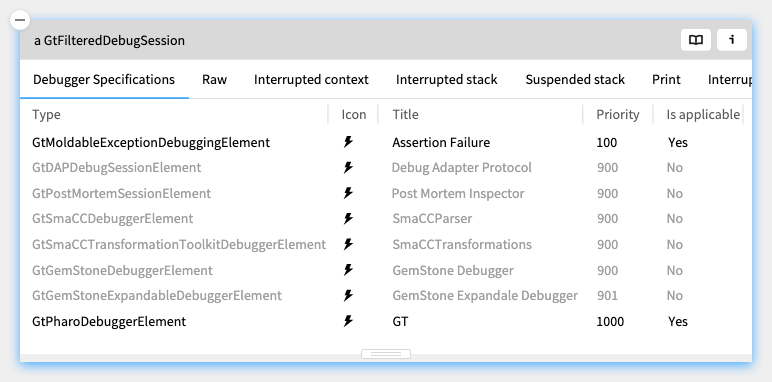
\includegraphics[width=\columnwidth]{availableDebuggerSpecifications}
  \caption{A list of debugger specifications found when an exception is raised.}
  \label{fig:availableDebuggerSpecifications}
\end{figure}

To enable moldable exceptions to perform automated transformations instead of opening the debugger, we provide a dedicated trait~\cite{Duca06b} that exceptions can use.
This trait provides an implementation for the signal method shown below.
This method is executed whenever an exception is raised.
By default in case an exception is not handled in the system a debugger is opened.
This override checks if automatic transformations are allowed for the current exception, and if they are, asks the exception for its transformation and executes it if there is anything to transform.
Transformations can apply code changes, modify the state of objects, or perform other operations, such as deleting no longer needed files.

\begin{code}
TGtMoldableExceptionSignalWithTransformation>>signal
	| transformation |
	self canApplyAutomaticTransformation
		ifFalse: [ ^ super signal ].
	transformation := self gtMoldableExceptionTransformation.
	transformation shouldTransform
		ifFalse: [ ^ self signal].
	transformation performTransformation
\end{code}

% ============================================================
\section{Discussion and future directions}\label{sec:directions}

Moldable exceptions are just objects augmented with annotated methods that create alternative views and actions when they are used to spawn a moldable debugger.
The previous extension mechanism for the moldable debugger required developers to extend the debugger by creating subclasses.
While both the moldable debugger and moldable inspector were available in Glamorous Toolkit at the same time, until now Glamorous Toolkit comes with 3200 views and 280 actions with an average of 12 lines of code, but only 8 custom debuggers (such as the one in  \autoref{fig:smaccDebugger}).

This indicates that the extension mechanism plays a significant role in developers extending the IDE, and that the cost of creating views and actions can be very low.
Due to this, through moldable exceptions we aim to apply the same extension mechanism present in the moldable inspector for creating custom debuggers.

At the time of writing we have implemented some 26 custom debugger views, in an average of under 12 lines of code.
Over half of these are forwarding views that reuse (delegate to) existing views previously defined as object inspector views.
Several more are simple text, list or tree views, and only three create custom graphical widgets.

The simplest debugging views are just like inspector views, and many of our examples just forward (delegate) to existing views, but more generally exceptions have access to the reified run-time stack at the time that they are raised, so debugger views can extract and present arbitrary run-time information.
The \emph{Scripter steps} view we saw earlier in \autoref{fig:scripterStepsViewClicked} offers an example.
The same approach could be used, for example, to present or highlight just the ``interesting'' stack frames, for example in an event-driven application, just the methods that are responsible for processing events.

At this time, moldable exceptions only offer the possibility to provide alternative views and actions, but not alternative ways to step through the execution.
Currently this is only possible in our setting by providing a completely separate debugger implementation.
In \autoref{fig:smaccDebugger} we see such a dedicated debugger for SmaCC~\cite{Brant17a}, the Smalltalk compiler compiler framework that has been spawned on an invalid fragment of Java code.
\begin{figure}[h]
  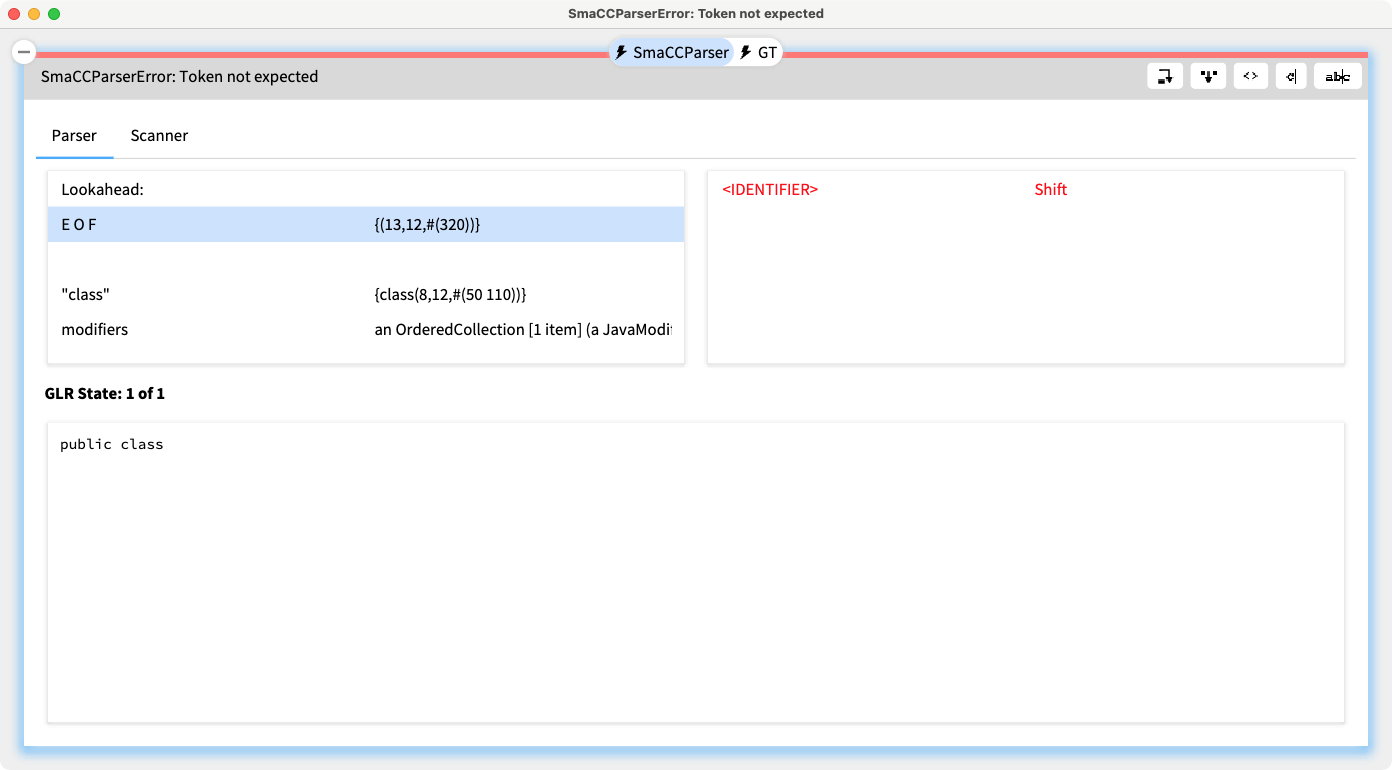
\includegraphics[width=\columnwidth]{smaccDebugger}
  \caption{A custom SmaCC debugger on an invalid Java snippet.}
  \label{fig:smaccDebugger}
\end{figure}
The SmaCC debugger offers the possibility to step through the grammar rules of a parser and explore its execution state.

Our proof-of-concept implementation of moldable exceptions presented here heavily leverages the existing infrastructure for moldable inspector views in \GT, but in principle there is nothing to prevent its application to other programming languages and IDEs.
The basic idea is simple: any moldable tool must be prepared, whenever it is created, to examine the execution context of the objects it is initialized with, and use that context to adapt its behavior.
In the case of a moldable debugger, this context is provided by the exception raised.
Custom debugger views and actions must then be provided by the specific exception raised.
One way to provide such views and actions is through specially annotated methods, but other means could be used, such as naming conventions, or a registry of debugger extensions.
The precise extension method will depend on the language technology available.

%\ac{As a side note.
%Technically we have access to the raised exception just when initially opening the debugger.
%Any step over action for example could lead to another exception being raises.
%The standard behaviour in Pharo is to always open the debugger on an exception.
%The default one is OupsNullException, but also in case an exception was explicitly raised doing a step into for example, changes the exception to the default one.
%I think we should more or less also do that.
%Currently we never change the exception that was raised in the debugger, even if when stepping we get another one.
%Just we can extend that with the notion of the last “real” exception that was raised, and a history of exceptions raised in that debugging session.
%Like that we could have step actions/view added by an exception that can be use as long as another explicit exception was not raised.}
%\on{Can you write a paragraph explaining this?}

% ============================================================
\section{Related work}\label{sec:related}

Early debuggers provided a command-line interface to inspect and step through the execution of a running program or a \emph{post mortem} ``core dump.''
With the advent of GUI-based IDEs, debuggers were also updated to offer interactive views to explore the execution state of a program and to step through its execution~\cite{Rose96a}.

% Debugging behavior
Studies of developer debugging behavior have shown that many developers have difficulty using debuggers and often shy away from them.
% Debugging: a review of the literature from an educational perspective
McCauley \etal report:
``We note, however, that our experiences with debugging tools is that many of them use execution traces as a method of assisting students to understand the execution of a program.
Tubaishat~\cite{Tuba01a} characterized the use of execution traces as an example of a shallow reasoning technique''~\cite{McCa08a}.
% On the Dichotomy of Debugging Behavior Among Programmers
And Beller \etal note that
``Debuggers are difficult to use.
Another reason given by interviewees, even though seasoned engineers, was that `the debugger is a complicated beast' (I2) and that `debuggers that are available now are certainly not friendly tools and they don't lend toward self-exploration'.''
\cite{Bell18a}

% Extensible debuggers
% A Simple and Extensible Graphical Debugger
An early example of an extensible debugger is \deet~\cite{Hans97a}.
Extensions to \deet were written Tcl/Tk or the Korn shell.
The focus of the extension mechanism in \deet is on adding new debugger features, rather than providing debugging support for specific application contexts.

The Java Virtual Machine Tools Interface (JVMTI)~\cite{JVMTI24} is an API for tools to inspect the state and control the execution of Java applications.
Agents can be written in any native language that supports C calling conventions.
Custom views must be built from scratch and integrated in your environment.

The VSCode Debugger Adapter Protocol (DAP)~\cite{DAP21} makes it possible to implement a generic debugger for a development tool that can communicate with different debuggers via Debug Adapters.

% Extensible Debugger Framework for Extensible Languages
mbeddr~\cite{Voel17a} is a collection of languages and language extensions, mainly focusing on C, built with the JetBrains MPS language workbench~\cite{Camp14a}.
mbeddr includes an extensible debugger framework~\cite{Pavl15a} that focuses on providing support for the individual language extension, not application specific customizations.

% [1] Omniscient Debugging for Executable DSLs
% https://inria.hal.science/hal-01662336/file/jss17-debugging.pdf
% [2] Protocol-Based Interactive Debugging for Domain-Specific Languages
% https://hal.science/hal-04124727/document
Bousse \etal have developed a generic omniscient (``back in time'') debugger that can be adapted to different domain-specific languages (DSLs) with moderate effort~\cite{Bous18a}.
They use DAP to provide new controls for DSLs in VSCode~\cite{Enet23a}.
Their work focuses more on the stepping semantics than on providing custom views.

% DSL Debugger extensions
There have been numerous efforts to develop specialized debuggers for DSLs using a variety of approaches.
%  Grammar-Driven Generation of Domain-Specific Language Debuggers
Wu \etal report on grammar-driven generation of DSL debuggers~\cite{HuiW08a}.
% Declaratively Defining Domain-Specific Language Debuggers
Lindeman \etal leverage the Spoofax language workbench~\cite{Kats10a} to declaratively define DSL debuggers~\cite{Lind11a}.
% D2X: An eXtensible conteXtual Debugger for Modern DSLs
D2X~\cite{Brah23a} provides an API for DSLs to define debugger extensions.
All of these DSL debugger approaches focus on providing general debugging for a given DSL, not for more finely-grained application debugging issues.

% Sindarin: A versatile scripting API for the Pharo debugger
Sindarin is an extensible Pharo-based debugger that offers a rich API for scripting debugger extensions~\cite{Dupr19a}.
The use case for Sindarin is rather different from that of moldable exceptions, allowing developers to enter debugger scripts during a debugging session, rather than as a way to enable specialized debugger behavior in response to specific kinds of exceptions.
It would be interesting to explore the use of Sindarin to implement custom stepping behavior.

% Moldable tools
The Moldable Debugger~\cite{Chis15c} is an example of a moldable tool~\cite{Chis17a} that adapts its behavior to a specific run-time application context.
The original moldable debugger, however, still required some significant implementation effort to define an alternative debugger interface, much like the other approaches we have cited from literature.
Similarly, the original moldable inspector~\cite{Chis15a} did not offer a very easy mechanism to provide custom inspector views depending on the object being inspected.
The adoption of the extension mechanism of using annotated methods to define inspector customizations led, over time, to the development of a large number of custom inspector views in the current version of \GT (over 3000 at last count).

% Historical
% Disciplined Exceptions
Disciplined use of exceptions is a well-established practice in object-oriented software development~\cite{Meye88a}.
The key insight and original contribution of moldable exceptions is to leverage exceptions as the hook to molding the behavior of the debugger.
Although it is common practice to add textual descriptions to exceptions, for example, by overriding the \st{toString()} method in Java, associating debugging views to exceptions is novel.
No previous approach to extensible debuggers, including the original moldable debugger, has taken this approach.

% ============================================================
\section{Conclusion}\label{sec:conclusion}

Debuggers are unloved beasts.
They provide a generic and low-level interface to explore and debug the run-time state of a running program.
Many debugging problems can be better tackled by understanding the nature of the exception that was raised and caused the debugger to be activated.
Our key contribution is to show how a debugger can be dynamically molded with custom views and actions that depend on the specific exception raised.
The mechanism is lightweight, and many useful extensions can be defined with minimal implementation effort.

%\begin{acks}
%Many thanks to Alexandre Bergel, Steven Costiou, and Timo Kehrer for their reviews of a draft of this paper.
%\end{acks}

\bibliographystyle{ACM-Reference-Format}
\bibliography{moldableExceptions}


\end{document}
\endinput


\begin{inparaenum}[(i)]
	\item ...
\end{inparaenum}
